\apendice{Documentación de usuario}

\section{Introducción}
En este anexo se va a realizar un manual de usuario detallado en el que se describa el uso de las diferentes características que ofrece el \textit{software} desarrollado de una forma sencilla para que cualquier persona sea capaz de entenderlo y poder utilizar la aplicación con normalidad, reduciendo la curva de aprendizaje que habría si no se tuviese este manual.

\section{Requisitos de usuarios}
Al tratarse de una aplicación web, los requisitos necesitados no son demasiados.
El usuario final de la aplicación tan solo necesita contar con un dispositivo con acceso a internet (en caso de tener la aplicación desplegada en un servidor externo a la red del dispositivo) y un navegador web con JavaScript habilitado.

El \textit{software} desarrollado cuenta con un correcto funcionamiento, al menos, bajo cualquiera de los siguientes navegadores:

\begin{enumerate}
\item Google Chrome (probado bajo la versión 114.0.5735.135).
\item Mozilla Firefox (probado en la versión 114.0.2).
\item Microsoft Edge (probado en la versión 114.0.1823.58).
\item Safari (probado en la versión 16.4).
\item Opera (probado en la versión 100.0.4815.21).
\end{enumerate}

\section{Instalación}
Al tratarse de una aplicación web no precisa de instalación, tan solo se debe acceder a la URL bajo la que se encuentre desplegada la aplicación. 
A la hora de realizar este trabajo, la URL de acceso es \url{https://flask-ubu.herokuapp.com/}

\section{Manual del usuario}
El siguiente manual de usuario se va a realizar con un usuario con permisos de modificación para poder mostrar todas las características de la web.
En caso de contar con un usuario con únicamente permisos de lectura, se mostrará parte de la información que aparece en este manual y otros elementos se encontrarán ocultos.

\subsection{Inicio de sesión}

Para comenzar a utilizar la aplicación lo primero que se debe hacer es acceder a la URL\footnote{A día de realización del trabajo: \url{https://flask-ubu.herokuapp.com/}} de la aplicación.

Al acceder a la dirección de la web por primera vez, se mostrará la página de inicio de sesión (ver figura~\ref{pag:login}) desde donde se debe indica el correo electrónico y la contraseña de la cuenta a utilizar.
La cuenta de correo y la contraseña debe ser la misma que la utilizada en el Moodle de la universidad.

\begin{figure}
	\centering
	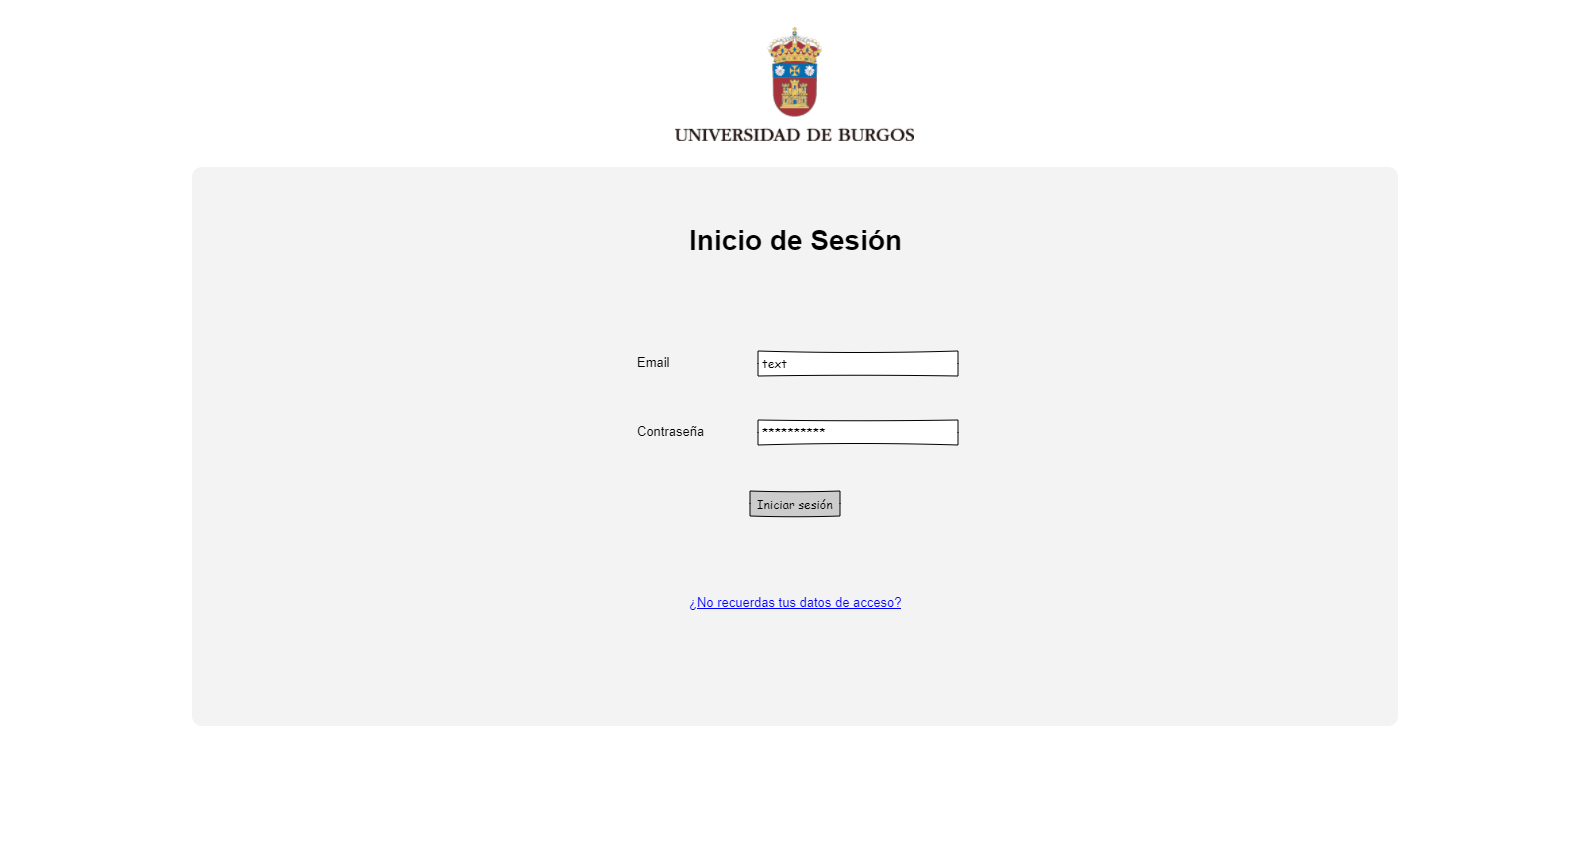
\includegraphics[width=\textwidth]{../img/Anexos/Manual usuario/login.png}
	\caption{Página de inicio de sesión}\label{pag:login}
\end{figure}

Si los datos de acceso son correctos, se tendrá acceso a la aplicación y se mostrará la página principal (imagen~\ref{pag:inicio}).
Una vez se tiene acceso a esta página, se puede acceder al resto de recursos de la web a través del menú superior de navegación.

\begin{figure}
	\centering
	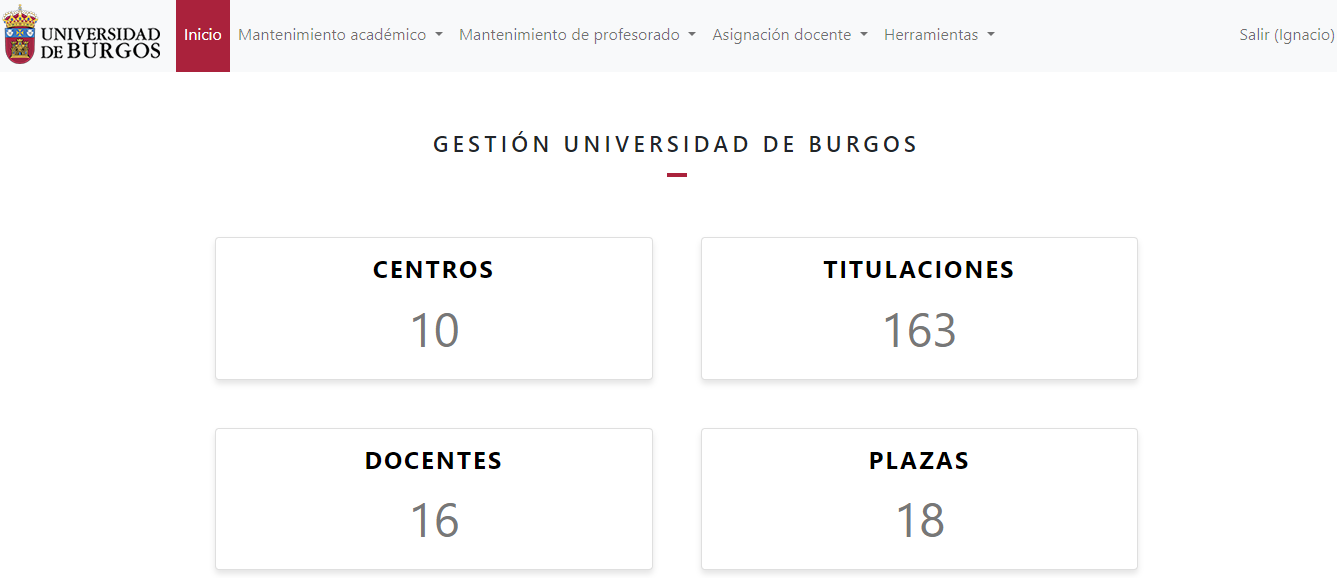
\includegraphics[width=\textwidth]{../img/Anexos/Manual usuario/inicio.png}
	\caption{Página principal}\label{pag:inicio}
\end{figure}

\subsection{Mantenimiento académico}
A continuación se van mostrar las diferentes funcionalidades dentro del mantenimiento académico de la aplicación.
Para ello, se debe pulsar sobre la opción del menú llamada <<Mantenimiento académico>> desde la que se desplegarán las opciones disponibles dentro de esta (imagen~\ref{pag:menuManAc}), las cuales son <<Centros>>, <<Titulaciones>> y <<Asignaturas>>.
Desde cada una de estas opciones se podrá realizar la visualización, creación y actualización de cada uno de estos componentes.

\begin{figure}
	\centering
	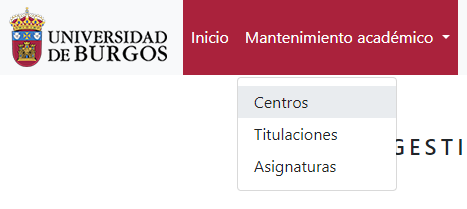
\includegraphics[width=\textwidth]{../img/Anexos/Manual usuario/menu man ac.png}
	\caption{Menú: Mantenimiento académico}\label{pag:menuManAc}
\end{figure}

\subsubsection{Creación de centros}
Pulsando sobre la opción del menú <<Centros>> se accede a la vista principal de los centros de la aplicación (imagen~\ref{pag:centros}).
Para crear un nuevo centro se debe pulsar sobre el botón <<Nuevo>> lo que provocará una redirección a la página que contiene el formulario de creación de centros (imagen~\ref{pag:formCentro}).

\begin{figure}
	\centering
	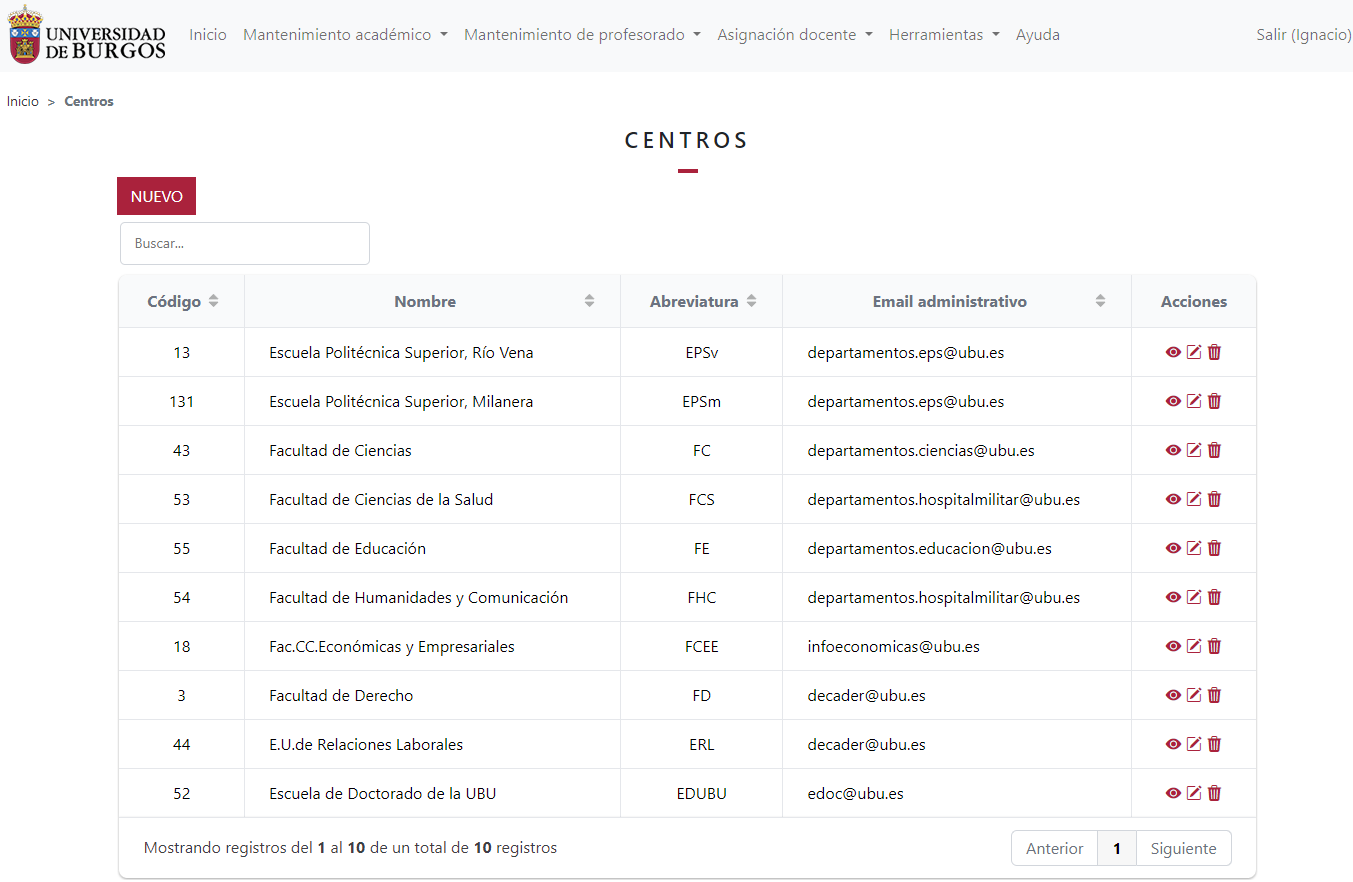
\includegraphics[width=\textwidth]{../img/Anexos/Manual usuario/centros.png}
	\caption{Página principal de centros}\label{pag:centros}
\end{figure}

\begin{figure}
	\centering
	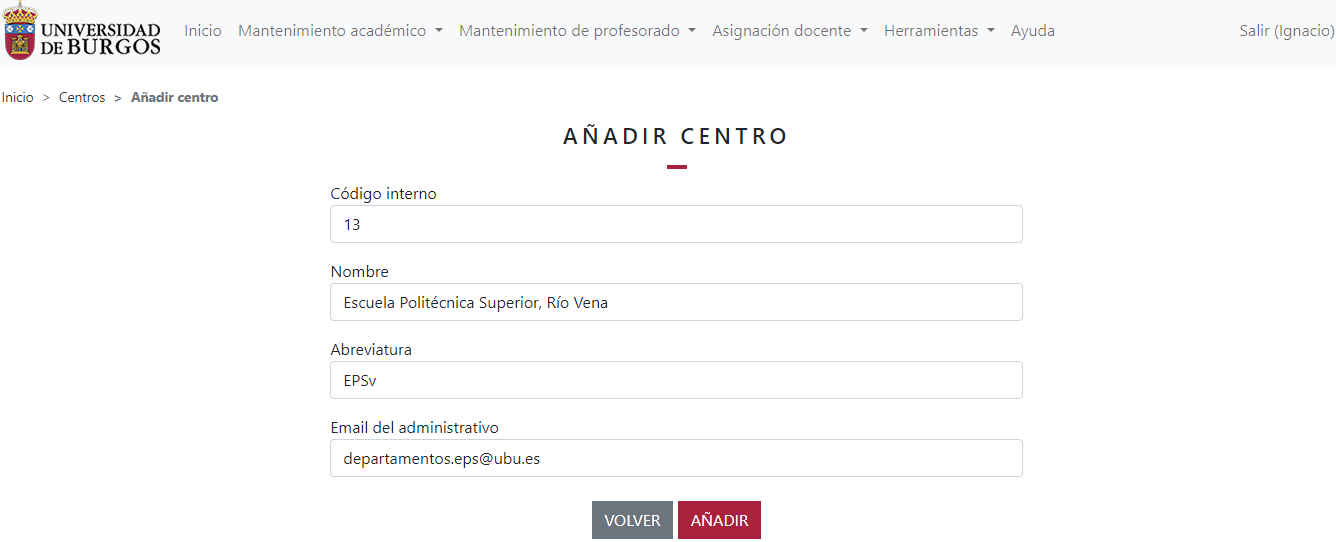
\includegraphics[width=\textwidth]{../img/Anexos/Manual usuario/formCentro.png}
	\caption{Formulario de creación de centros}\label{pag:formCentro}
\end{figure}

Desde la página del formulario se deben rellenar los campos con los datos del nuevo centro y pulsar sobre el botón <<Añadir>>.
Esto provocará que el centro se almacene en la base de datos. 
La aplicación redirigirá al usuario a la página principal de centros (imagen~\ref{pag:centros}) mostrando un mensaje que indica la correcta creación del centro.

\subsubsection{Modificación de centros}
Desde la página principal de centros (imagen~\ref{pag:centros}), se debe pulsar, en la tabla, sobre el icono del lápiz del centro que se desea modificar.
Esta acción provocará la redirección a la página del formulario de modificación, que contendrá los datos del centro seleccionado (imagen~\ref{pag:formModCentro}).

Desde esta página se pueden modificar los campos deseados y, al finalizar, pulsar sobre el botón <<Modificar>>.
Esta acción producirá una redirección a la página principal de centros, mostrando un mensaje que indica la correcta modificación del centro.

\begin{figure}
	\centering
	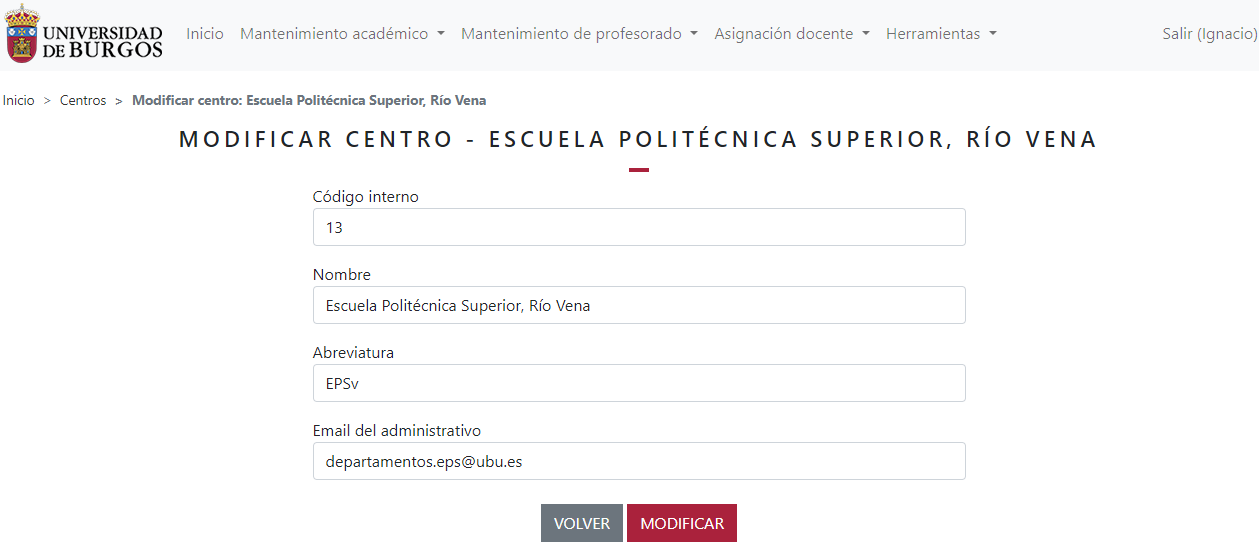
\includegraphics[width=\textwidth]{../img/Anexos/Manual usuario/formModCentro.png}
	\caption{Formulario de modificación de centros}\label{pag:formModCentro}
\end{figure}

\subsubsection{Eliminación de centros}
Desde la página principal de centros se puede eliminar un centro pulsando sobre el icono de la papelera del centro de la tabla que se desea eliminar.
Al hacer esto se mostrará la alerta de la imagen~\ref{pag:alertElCentro} y pulsando sobre el botón <<Aceptar>>, se realizará la petición de eliminación del centro.

Al hacer esto se mostrará un mensaje indicando la correcta eliminación o un mensaje indicando que no se ha podido realizar la eliminación en caso de que el centro tenga titulaciones asociadas.

\begin{figure}
	\centering
	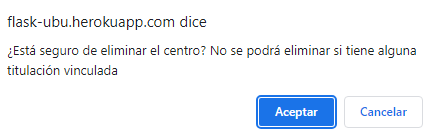
\includegraphics[width=\textwidth]{../img/Anexos/Manual usuario/alertElCentro.png}
	\caption{Alerta de eliminación de centros}\label{pag:alertElCentro}
\end{figure}

\subsubsection{Creación de titulaciones}
Pulsando sobre la opción del menú <<Titulaciones>> se accede a la vista principal de las titulaciones (ver imagen~\ref{pag:titulaciones}).

Para crear una nueva titulación se debe pulsar sobre el botón <<Nuevo>>.
Es importante tener en cuenta que para crear una titulación es necesario tener un centro creado previamente, ya que una titulación se vincula a un centro.

\begin{figure}
	\centering
	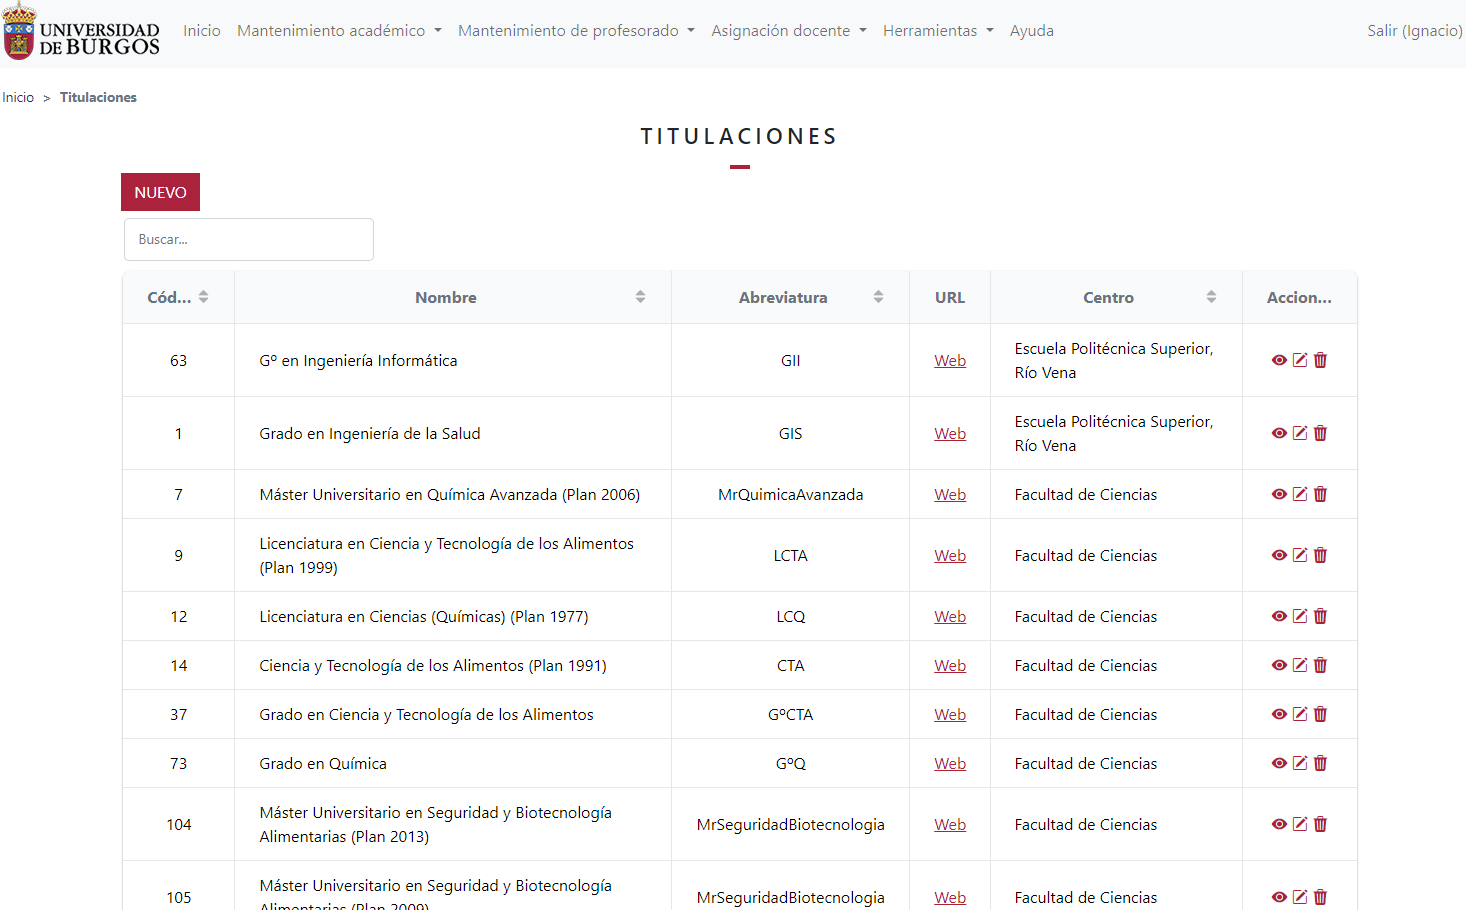
\includegraphics[width=\textwidth]{../img/Anexos/Manual usuario/titulaciones.png}
	\caption{Página principal de titulaciones}\label{pag:titulaciones}
\end{figure}

Al pulsar sobre el botón <<Nuevo>> se abre el formulario de creación de titulaciones.
Está página se puede ver en la imagen~\ref{pag:formTitulacion}.
En este formulario se deben introducir los datos de la titulación que se desea crear y, una vez se tengan los campos completados, pulsar sobre el botón <<Añadir>>.
Esta acción producirá una redirección a la página principal de titulaciones donde se podrá ver la titulación creada.
Además, se mostrará un mensaje indicando la creación de la titulación.

\begin{figure}
	\centering
	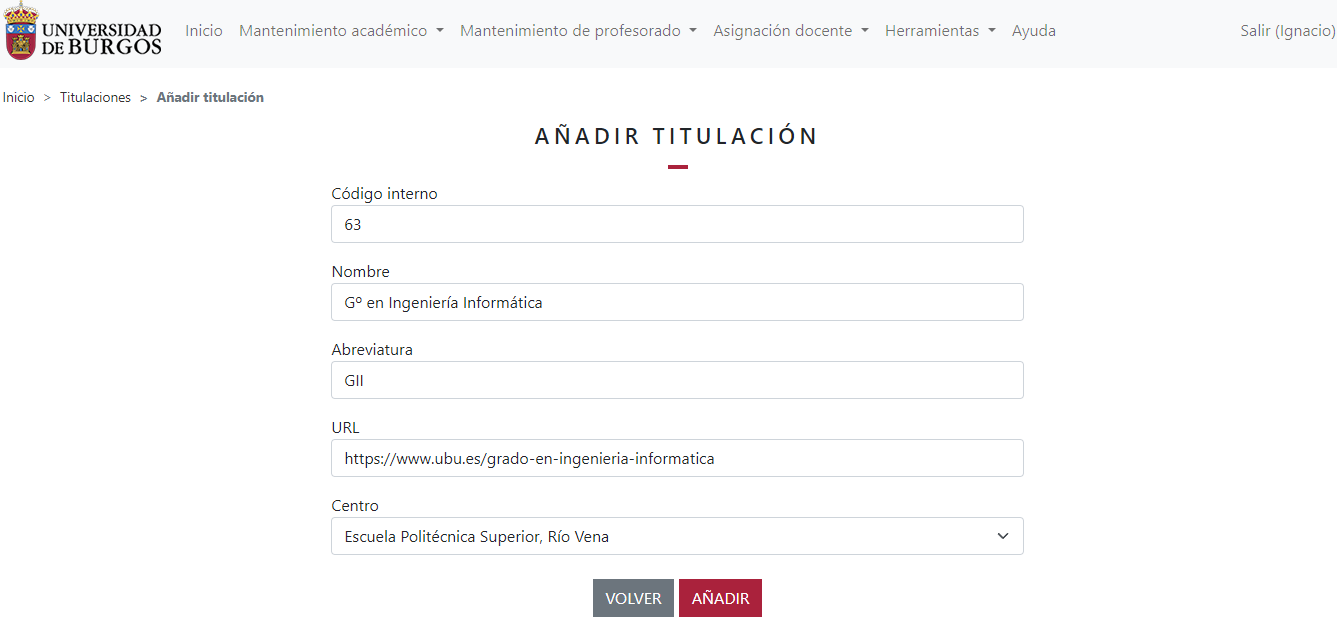
\includegraphics[width=\textwidth]{../img/Anexos/Manual usuario/formTitulacion.png}
	\caption{Formulario de creación de titulaciones}\label{pag:formTitulacion}
\end{figure}

\subsubsection{Modificación de titulaciones}
Para modificar una titulación, encontrándonos en la página principal de titulaciones (imagen~\ref{pag:titulaciones}), se debe pulsar sobre el icono de la lápiz de la titulación de la lista que se desea modificar.
Esto abrirá la página con el formulario de modificación de la titulación (ver imagen~\ref{pag:formModTitulacion}).

\begin{figure}
	\centering
	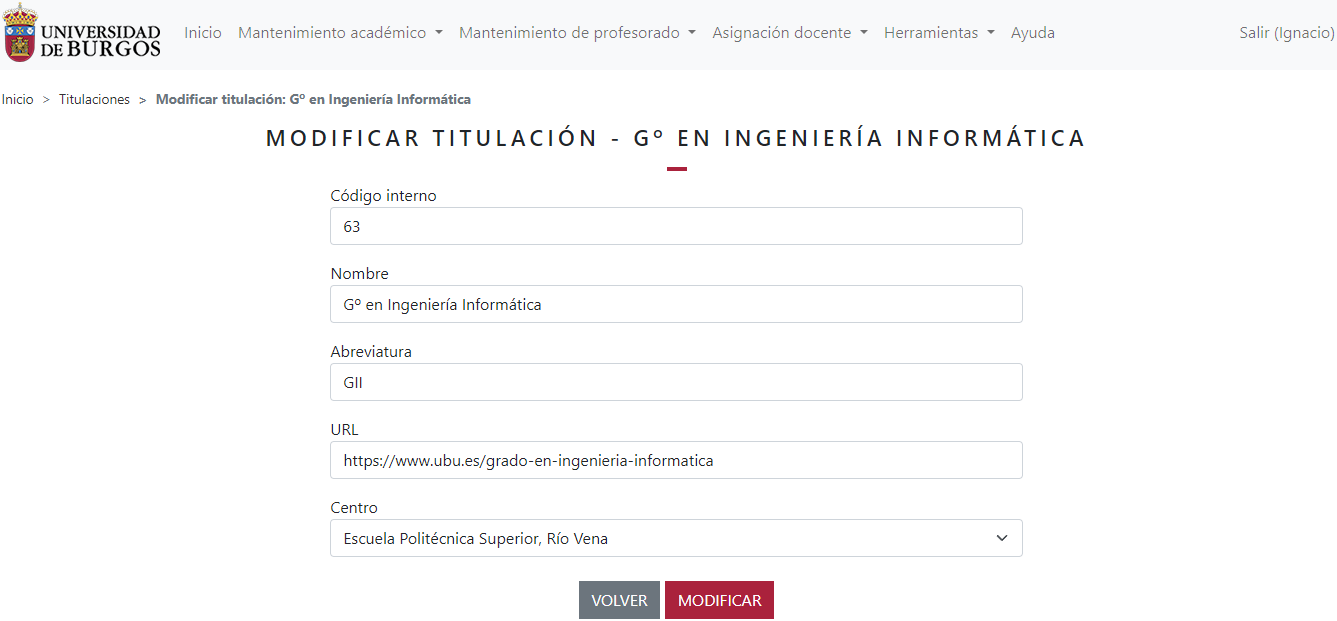
\includegraphics[width=\textwidth]{../img/Anexos/Manual usuario/formModTitulacion.png}
	\caption{Formulario de modificación de titulaciones}\label{pag:formModTitulacion}
\end{figure}

Desde este formulario se pueden modificar los campos deseados.
Una vez concluida la modificación se debe pulsar sobre el botón <<Modificar>>.
Esto plasmará los cambios en la base de datos y la web redirigirá al usuario a la página principal de titulaciones indicando mediante un mensaje la correcta modificación.

\subsubsection{Eliminación de titulaciones}
Desde la página principal de titulaciones (imagen~\ref{pag:titulaciones}), se debe pulsar sobre el icono de la papelera de la titulación que se desea eliminar.
Al realizar esta acción aparecerá en la pantalla la alerta de la imagen~\ref{pag:alertElTitulacion}. Si se pulsa sobre el botón <<Aceptar>> la titulación se eliminará de la base de datos si no tiene asignaturas asociadas, en caso contrario, no se podrá eliminar y aparecerá un mensaje de error mostrando esta información.

\begin{figure}
	\centering
	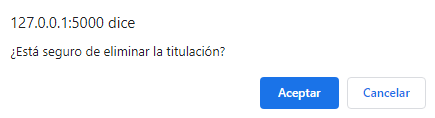
\includegraphics[width=\textwidth]{../img/Anexos/Manual usuario/alertElTitulacion.png}
	\caption{Alerta de eliminación de titulaciones}\label{pag:alertElTitulacion}
\end{figure}

\subsubsection{Creación de asignaturas}
Para añadir una nueva asignatura a la web, se debe pulsar sobre la opción del menú llamada <<Asignaturas>>.
Realizar esta acción redirige al usuario a la página principal de asignaturas (imagen~\ref{pag:asignaturas}).

Es importante tener en cuenta que previamente se debe haber creado la titulación a la que se quiere vincular la asignatura.

\begin{figure}
	\centering
	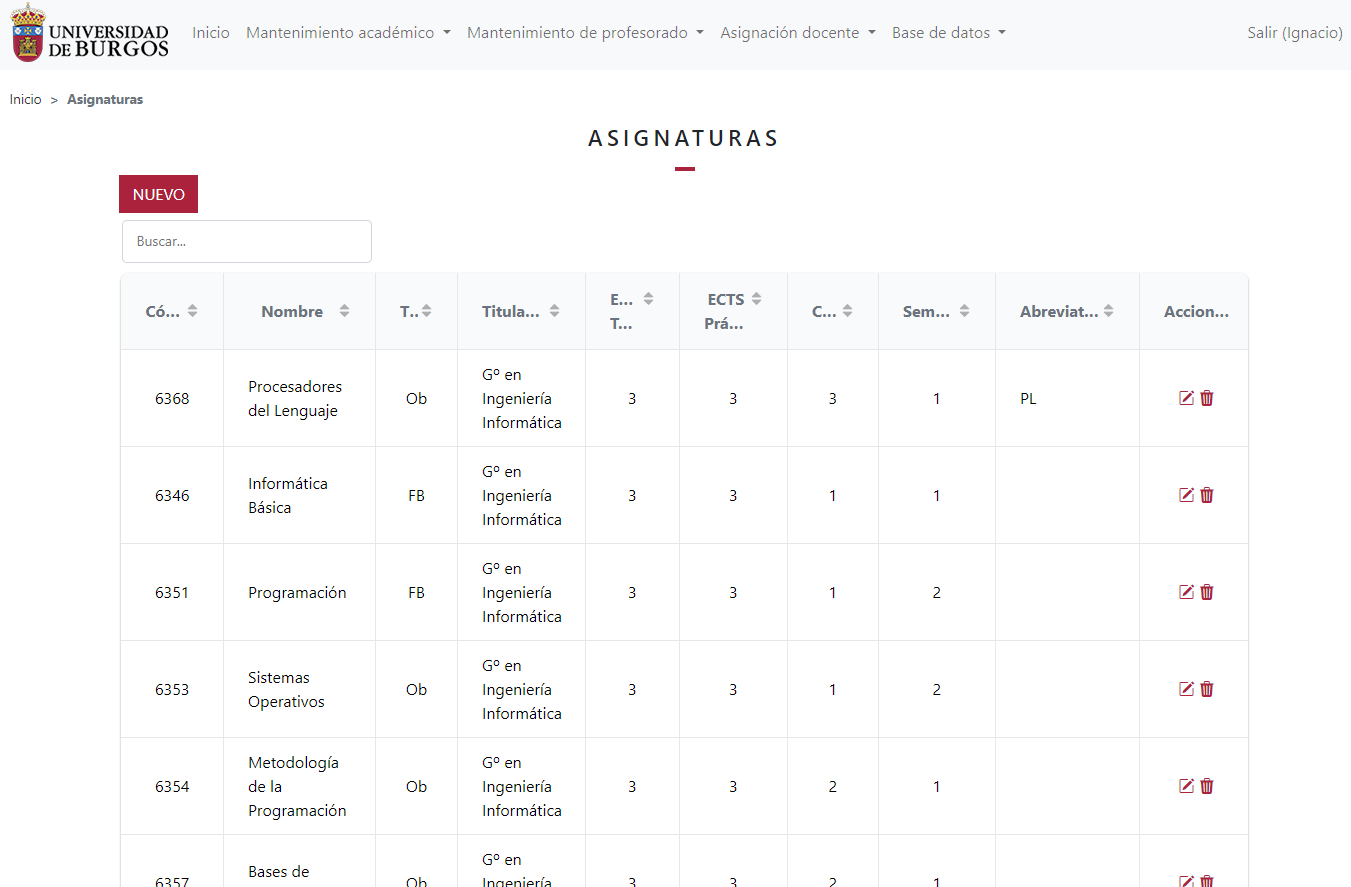
\includegraphics[width=\textwidth]{../img/Anexos/Manual usuario/asignaturas.png}
	\caption{Página principal de asignaturas}\label{pag:asignaturas}
\end{figure}

Una vez en la página principal de asignaturas se debe pulsar sobre el botón <<Nuevo>>, lo que abrirá el formulario de creación de asignaturas (ver imagen~\ref{pag:formAsignatura}).

Con los campos del formulario completados solo queda pulsar sobre el botón <<Añadir>> para almacenar la asignatura en la base de datos.
Tras realizar esta acción, se mostrará la página principal de asignaturas junto a un mensaje informando de la correcta creación de la asignatura.

\begin{figure}
	\centering
	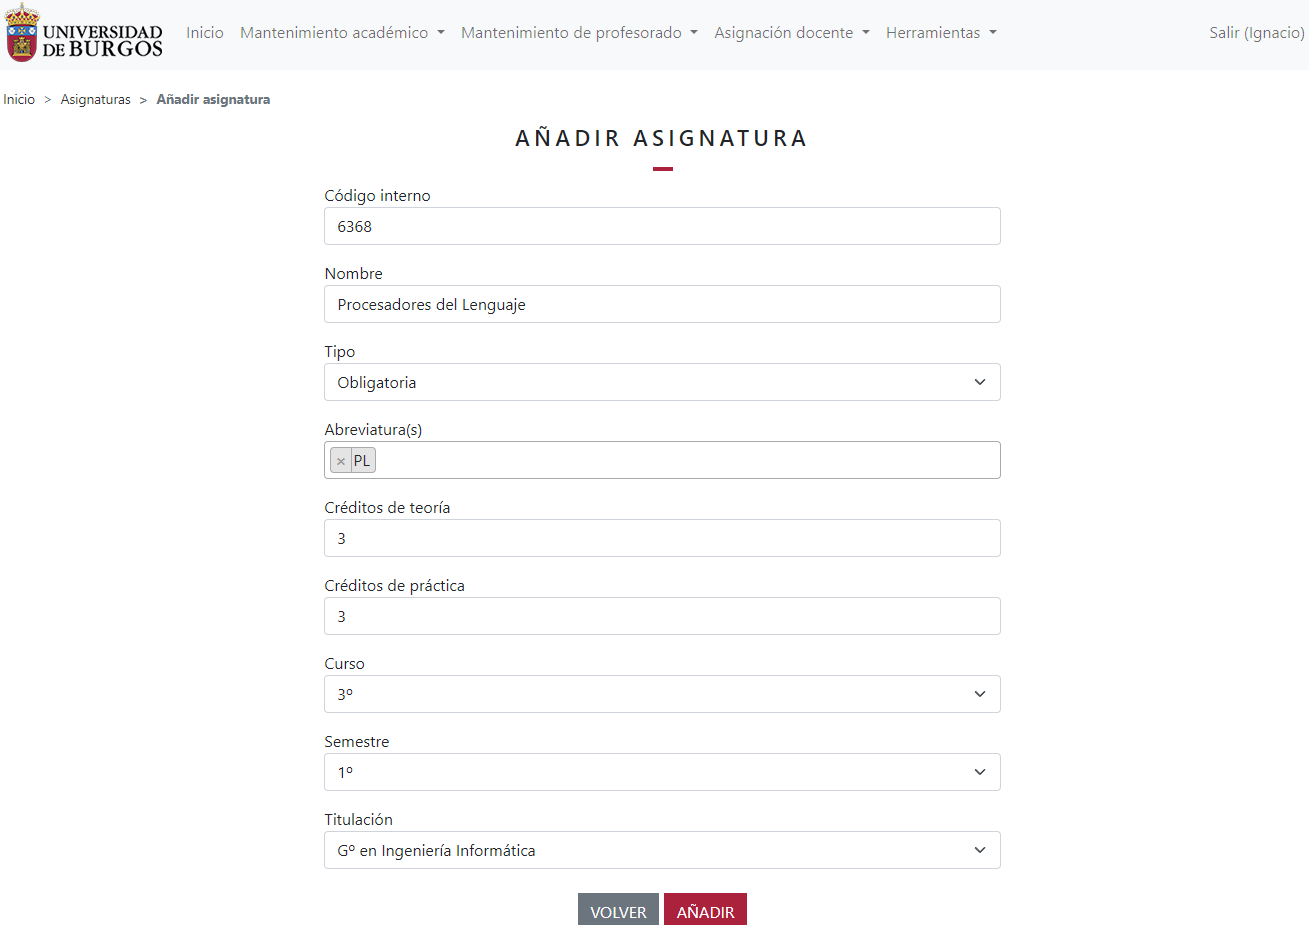
\includegraphics[width=\textwidth]{../img/Anexos/Manual usuario/formAsignatura.png}
	\caption{Formulario de creación de asignaturas}\label{pag:formAsignatura}
\end{figure}

\subsubsection{Modificación de asignaturas}
Para modificar una asignatura se debe pulsar sobre el icono del lápiz de la asignatura de la tabla que se desea modificar.
Esto abrirá el formulario de modificación de la asignatura con los campo rellenos con la información de la asignatura a editar (ver imagen~\ref{pag:formModAsignatura}).

En este momento se pueden editar los campos deseados y al finalizar, se debe pulsar sobre el botón <<Modificar>>.
Esto provocará el guardado de la información y una redirección a la página de asignaturas donde se mostrará un mensaje informativo sobre la modificación de la asignatura.

\begin{figure}
	\centering
	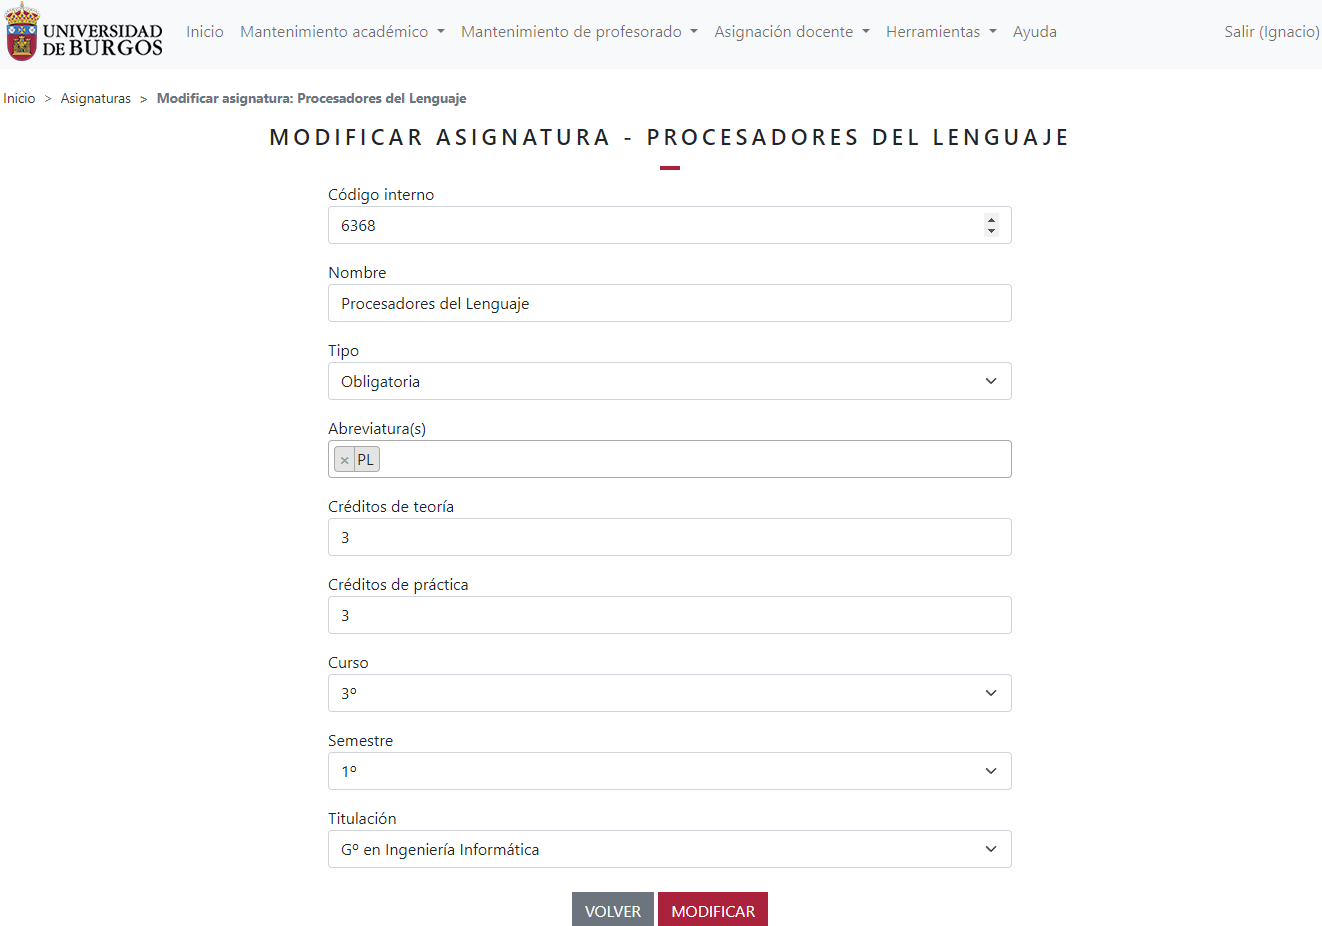
\includegraphics[width=\textwidth]{../img/Anexos/Manual usuario/formModAsignatura.png}
	\caption{Formulario de modificación de asignaturas}\label{pag:formModAsignatura}
\end{figure}

\subsubsection{Eliminación de asignaturas}
Si se desea eliminar una asignatura de la aplicación, se debe acceder a la página principal de asignaturas y, una vez aquí, pulsar sobre el icono de la papelera de la asignatura que se desea eliminar.

Al realizar la acción descrita, se abre una alerta de confirmación (ver imagen~\ref{pag:alertElAsignatura}).
Al pulsar sobre <<Aceptar>> la asignatura se elimina de la aplicación produciendo un borrado en cascada de sus relaciones con los cursos académicos creados.

\begin{figure}
	\centering
	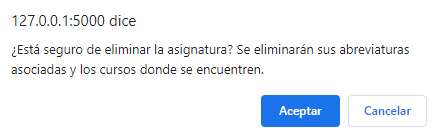
\includegraphics[width=.8\textwidth]{../img/Anexos/Manual usuario/alertElAsignatura.png}
	\caption{Alerta de eliminación de titulaciones}\label{pag:alertElAsignatura}
\end{figure}

\subsection{Mantenimiento de profesorado}
En esta sección se va a mostrar el manual de usuario sobre el mantenimiento de profesorado.
Esta parte de la aplicación incluye la creación, modificación y eliminación de los elementos que se pueden ver en la imagen~\ref{pag:menuManProf}.

\begin{figure}
	\centering
	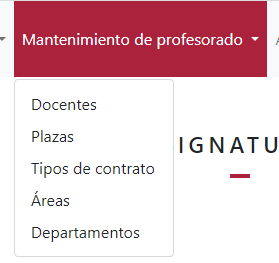
\includegraphics[width=.5\textwidth]{../img/Anexos/Manual usuario/menu man prof.png}
	\caption{Menú: Mantenimiento de profesorado}\label{pag:menuManProf}
\end{figure}

\subsubsection{Creación de docentes}
Para crear un nuevo docente, necesario para obtener acceso a la aplicación, se debe pulsar sobre la opción del menú llamada <<Docentes>>.
Esto abrirá la página principal de docentes (ver imagen~\ref{pag:docentes}).

\begin{figure}
	\centering
	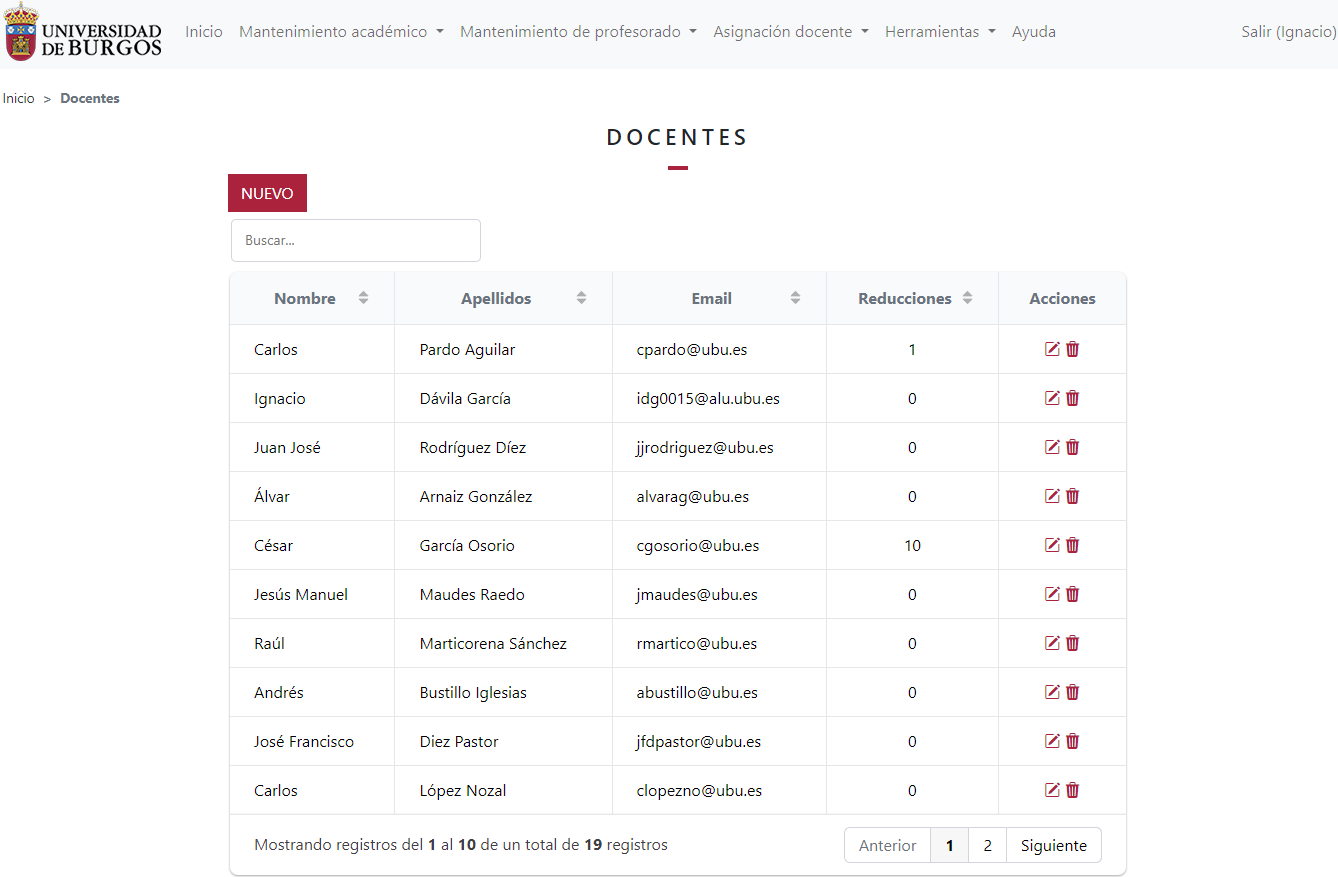
\includegraphics[width=\textwidth]{../img/Anexos/Manual usuario/docentes.png}
	\caption{Página principal de docentes}\label{pag:docentes}
\end{figure}

Desde esta página se debe pulsar sobre el botón <<Nuevo>>, lo que abrirá el formulario de creación de docentes (imagen~\ref{pag:formDocente}).

Una vez en la página del formulario, se deben rellenar los campos con los datos del docente que se desea añadir.
Es importante tener en cuenta que desde aquí se indican los permisos que tendrá el docente.
Si se le conceden permisos de modificación tendrá acceso a todas las funcionalidades descritas en este manual, mientras que si se le dan únicamente permisos de consulta, solo tendrá permiso para visualizar la información que administra la aplicación web.
Por último, en caso de no indicar ningún tipo de permiso, el usuario no tendrá acceso a la aplicación, aunque este dado de alta en el Moodle de la universidad.

\begin{figure}
	\centering
	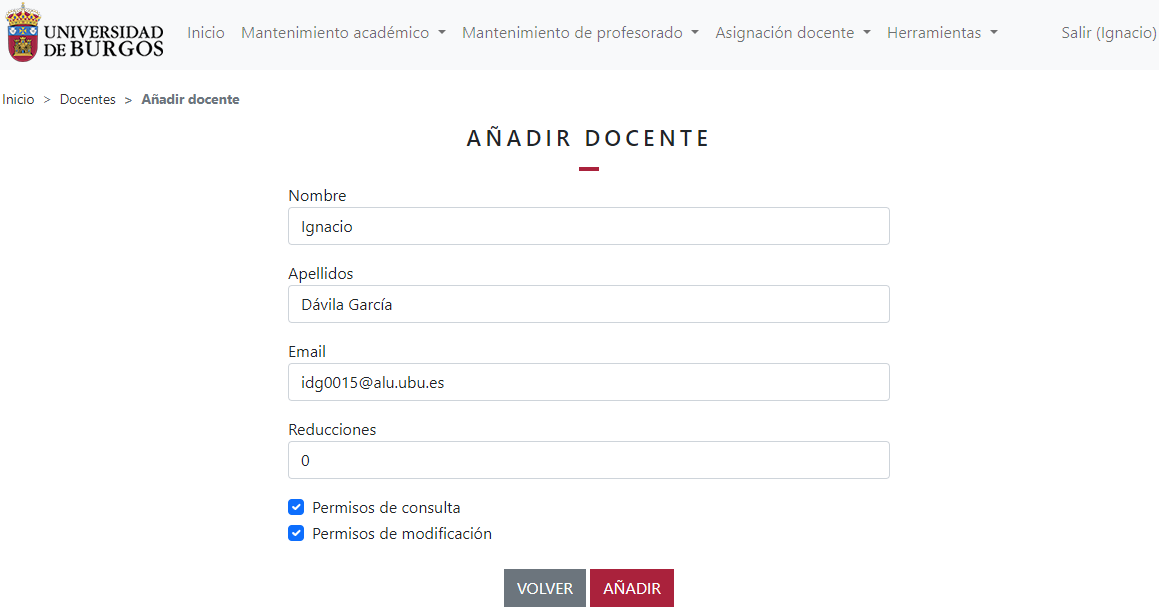
\includegraphics[width=\textwidth]{../img/Anexos/Manual usuario/formDocente.png}
	\caption{Formulario de creación de docentes}\label{pag:formDocente}
\end{figure}

\subsubsection{Modificación de docentes}
Para realizar la modificación de los datos de un docente se debe ir a la página principal de docentes (imagen~\ref{pag:docentes}).

Desde esta ventana se debe pulsar sobre el icono del lápiz del registro de la tabla correspondiente al docente que se desea modificar.
Esta acción producirá la redirección a la página del formulario de modificación del docente seleccionado, que se puede ver en la imagen~\ref{pag:formModDocente}.

\begin{figure}
	\centering
	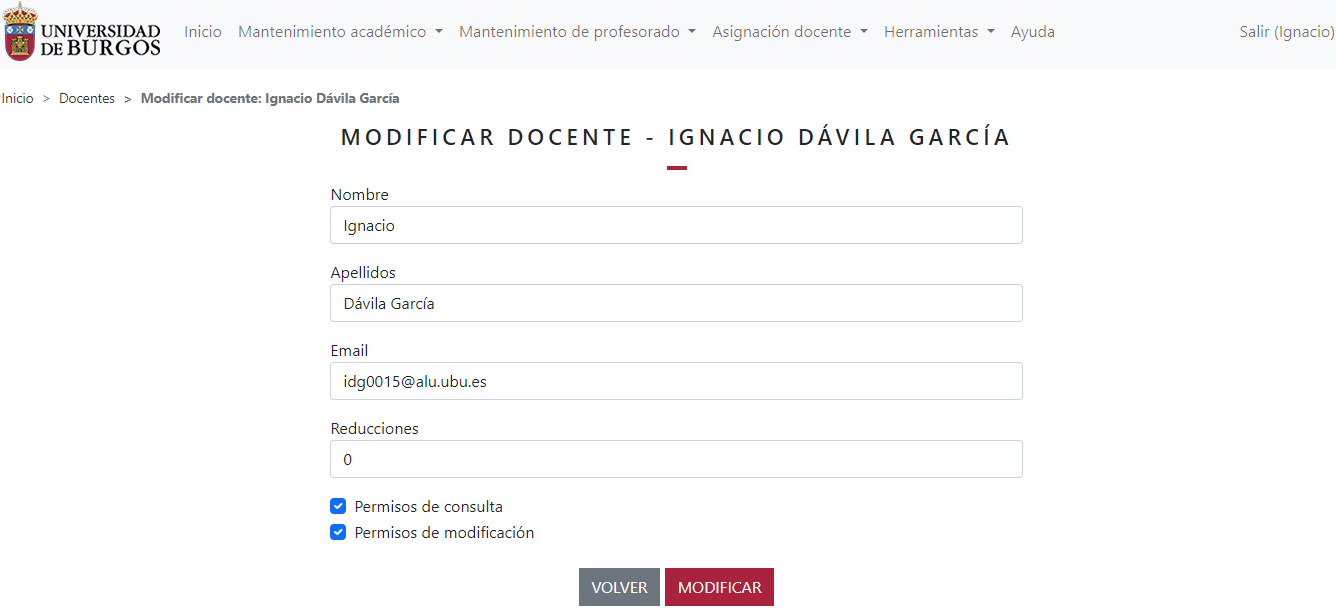
\includegraphics[width=\textwidth]{../img/Anexos/Manual usuario/formModDocente.png}
	\caption{Formulario de modificación de docentes}\label{pag:formModDocente}
\end{figure}

Una vez se hayan realizado los cambios deseados en los datos se debe pulsar sobre el botón de <<Modificar>>, lo que provocará la modificación en la base de datos de los datos y la redirección a la página principal de docentes donde se mostrará un mensaje indicando la correcta modificación.

\subsubsection{Eliminación de docentes}
Si se desea dar de baja de la base de datos a un docente se debe ir a la página principal de docentes donde se muestra una tabla con todos los que se encuentran dados de alta.
En esta tabla se debe buscar el docente a eliminar y pulsar sobre el icono de la papelera de la fila correspondiente al docente.

Tras realizar esta acción se abrirá una alerta de confirmación acerca de eliminar el docente.
Si se pulsa sobre <<Aceptar>> el docente desaparecerá de la base de datos y se podrá ver un mensaje indicando la correcta eliminación.

\subsubsection{Creación de plazas}
La creación de plazas se realiza accediendo a la página principal de plazas (imagen~\ref{pag:plazas}) al pulsar sobre la opción del menú <<Plazas>>.

\begin{figure}
	\centering
	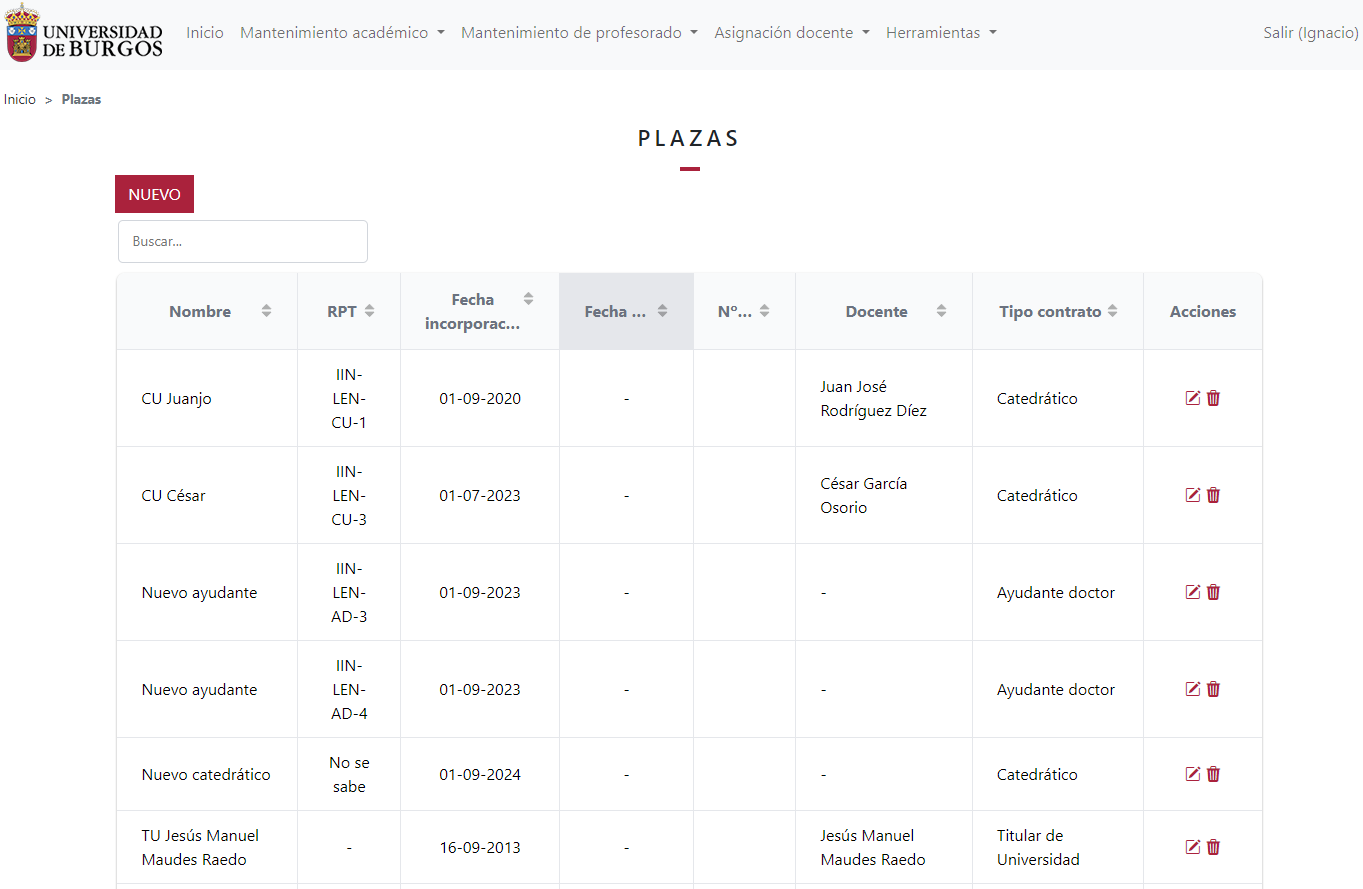
\includegraphics[width=\textwidth]{../img/Anexos/Manual usuario/plazas.png}
	\caption{Página principal de plazas}\label{pag:plazas}
\end{figure}

Desde esta ventana se debe pulsar sobre el botón <<Nuevo>>, lo que abrirá la página que contiene el formulario de creación de plazas (ver imagen~\ref{pag:formPlaza}).

\begin{figure}
	\centering
	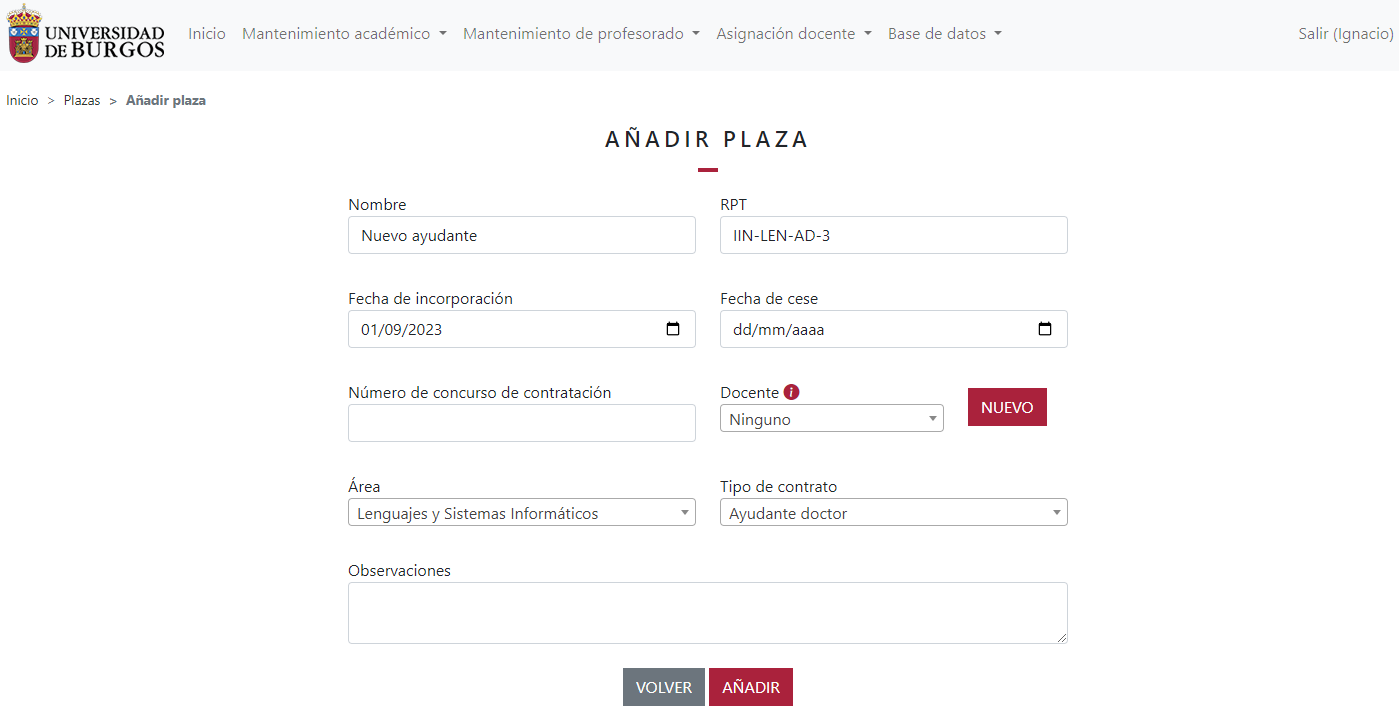
\includegraphics[width=\textwidth]{../img/Anexos/Manual usuario/formPlaza.png}
	\caption{Formulario de modificación de plazas}\label{pag:formPlaza}
\end{figure}

Desde está página se pueden completar los campos del formulario con los datos de la plaza que se desea dar de alta. 
Además, en caso de querer crear un docente en el mismo momento de creación de la plaza, se puede pulsar sobre el botón <<Nuevo>> del campo llamado <<Docente>>.
Esto abrirá una ventana modal con el formulario de creación de docentes (imagen~\ref{pag:formDocente}) desde el que se podrá crear el docente que después podrá ser seleccionado desde el formulario de plazas.

Es importante tener en cuenta de que para crear una nueva plaza es necesario tener creada previamente el área a la que pertenecerá la plaza y el tipo de contrato que tendrá.

Cuando se tengan todos los campos obligatorios completados, se debe pulsar sobre el botón <<Añadir>>.
Tras esta acción la web redirigirá a la página principal de plazas mostrando un mensaje informando sobre la creación de la plaza.

\subsubsection{Modificación de plazas}
Para realizar la modificación de los datos de una plaza se debe acceder a la página principal de plazas (figura~\ref{pag:plazas}).

Una vez en esa página se debe pulsar sobre el icono del lápiz de la plaza que se desea modificar.
Esto abrirá la página que contiene el formulario de modificación de plazas (imagen~\ref{pag:formModPlaza}) con todos los datos de la plaza disponibles para ser editados.

Una vez se tengan los campos deseados editados, se debe pulsar sobre el botón <<Modificar>>.
De esta manera la información quedará actualizada y seremos redirigidos a la página principal de plazas, donde se podrán ver reflejados los cambios. 
También se mostrará un mensaje informando de la modificación de la plaza.

\begin{figure}
	\centering
	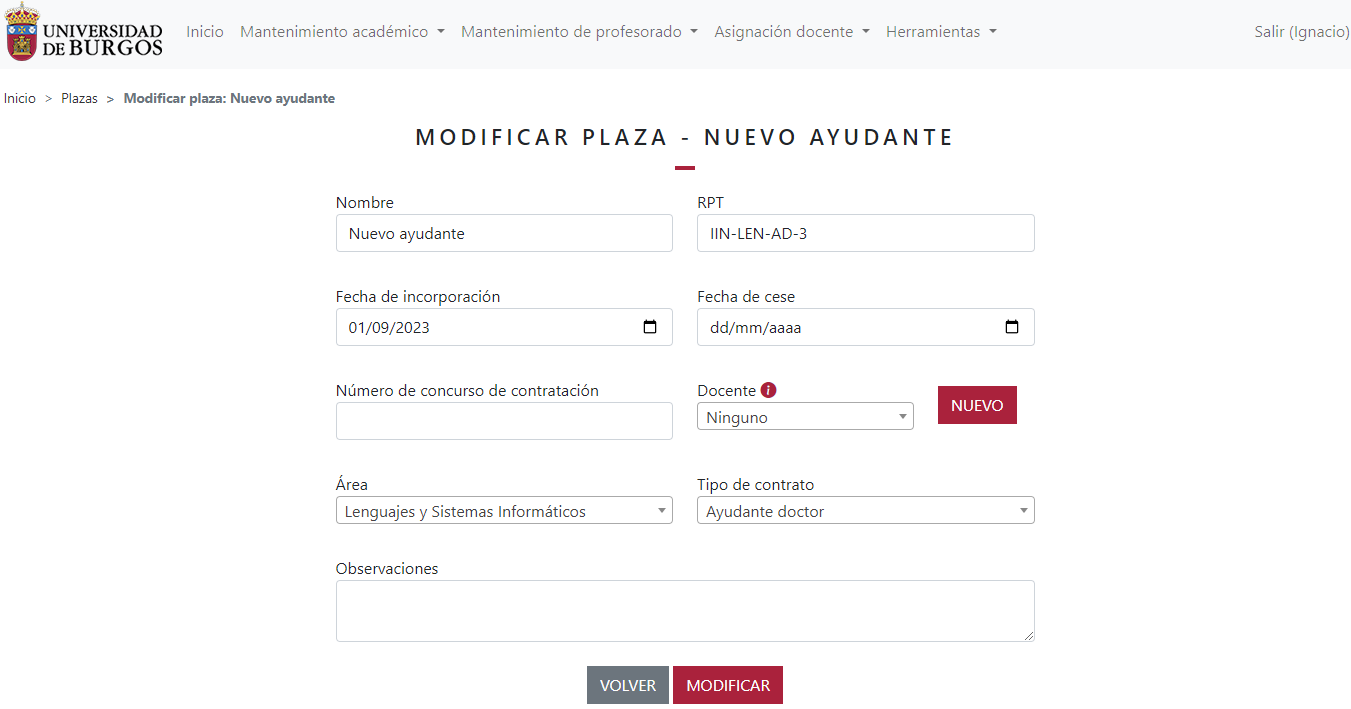
\includegraphics[width=\textwidth]{../img/Anexos/Manual usuario/formModPlaza.png}
	\caption{Formulario de modificación de plazas}\label{pag:formModPlaza}
\end{figure}

\subsubsection{Eliminación de plazas}
Si se desea eliminar una plaza que se encuentra en la aplicación web, se debe ir a la página principal de plazas y, desde esta página, se debe pulsar en el icono de la papelera de la plaza del listado que se desea eliminar.
Esta acción provocará la apertura de una alerta de confirmación como la de la figura~\ref{pag:alertElPlaza} en la que se informa de que, en caso de eliminar la plaza, se eliminarán con ella las posibles relaciones que tenga con grupos de las asignaturas del curso académico correspondiente.

Si se pulsa en <<Aceptar>> la plaza y sus vinculaciones quedan eliminadas, y se mostrará un mensaje informando de la eliminación.

\begin{figure}
	\centering
	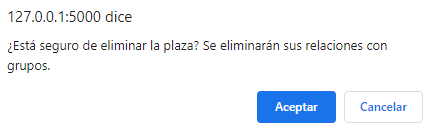
\includegraphics[width=.5\textwidth]{../img/Anexos/Manual usuario/alertElPlaza.png}
	\caption{Alerta de eliminación de plaza}\label{pag:alertElPlaza}
\end{figure}

\subsubsection{Creación de tipos de contrato}
En este apartado se va a mostrar la información necesaria para poder crear un nuevo tipo de contrato.

Para comenzar se debe pulsar la opción del menú <<Tipos de contrato>> que se encuentra dentro de <<Mantenimiento de profesorado>>.
Al realizar esta acción la web nos mostrará la pantalla principal de los contratos (ver imagen~\ref{pag:contratos}).

\begin{figure}
	\centering
	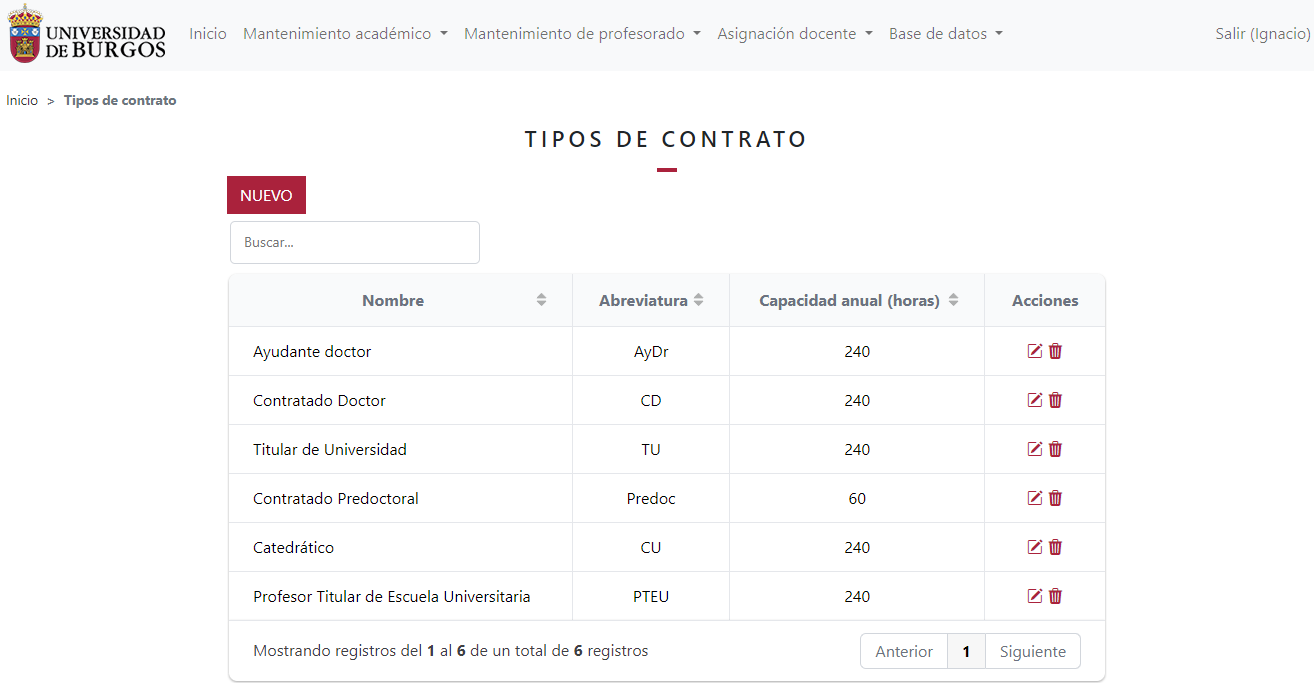
\includegraphics[width=\textwidth]{../img/Anexos/Manual usuario/contratos.png}
	\caption{Página principal de tipos de contrato}\label{pag:contratos}
\end{figure}

Para crear el nuevo tipo de contrato se debe pulsar sobre el botón <<Nuevo>> que aparece en la página, encima de la tabla.
Esto hará una redirección al formulario de creación de tipos de contrato (imagen~\ref{pag:formContrato}).

En este formulario se deben ingresar los datos del nuevo tipo de contrato que se desea crear.
Una vez se tenga el formulario completo hay que pulsar sobre el botón <<Añadir>>.
Al realizar esta acción, la página web nos redirigirá a la página principal de tipos de contrato.
Además, aparecerá un mensaje informando acerca de la creación del tipo de contrato.

\begin{figure}
	\centering
	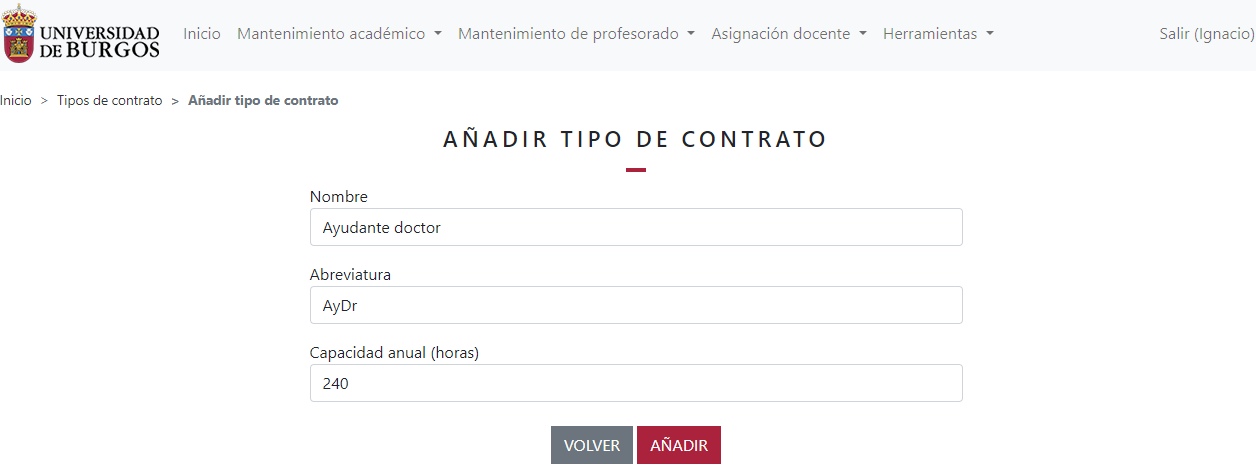
\includegraphics[width=\textwidth]{../img/Anexos/Manual usuario/formContrato.png}
	\caption{Formulario de creación de tipos de contrato}\label{pag:formContrato}
\end{figure}

\subsubsection{Modificación de tipos de contrato}
Si se desea modificar la información de un tipo de contrato se debe acceder a la página principal de tipos de contrato.

Desde esta página se debe buscar el tipo de contrato a modificar en la tabla y se debe pulsar sobre el icono del lápiz de la columna <<Acciones>>.
Al hacer esto la web nos llevará al formulario de modificación del tipo de contrato (ver imagen~\ref{pag:formModContrato}), que tendrá todos los campos rellenos con la información aportada a la hora de haberlo creado.

Cuando se hayan modificado los campos deseados se debe pulsar sobre el botón <<Modificar>>.
De esta manera la información quedará actualizada y volveremos a la página principal donde se mostrará un mensaje con información sobre la modificación realizada.

\begin{figure}
	\centering
	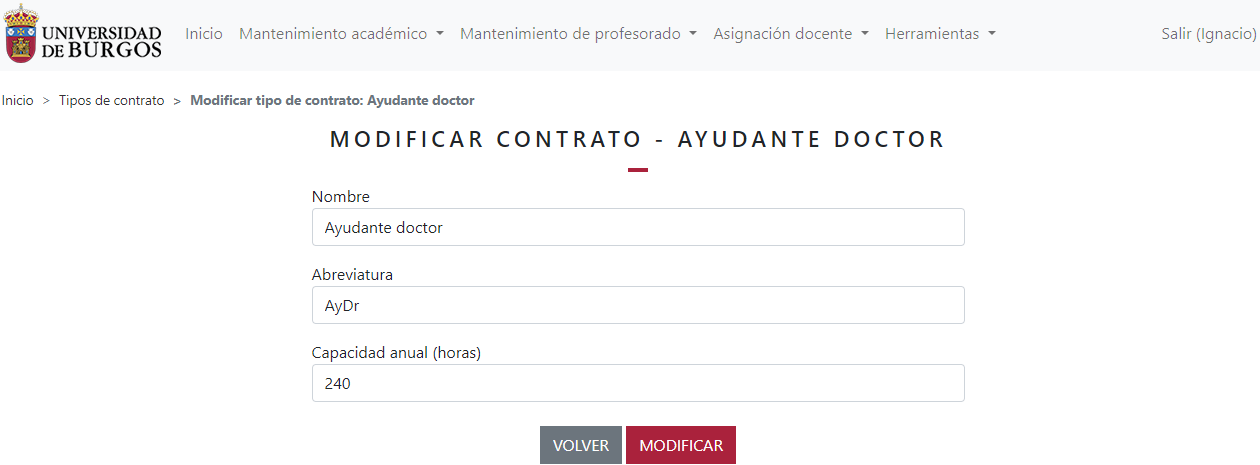
\includegraphics[width=\textwidth]{../img/Anexos/Manual usuario/formModContrato.png}
	\caption{Formulario de modificación de tipos de contrato}\label{pag:formModContrato}
\end{figure}

\subsubsection{Eliminación de tipos de contrato}
En este apartado se van a indicar los pasos necesarios para realizar la eliminación de un tipo de contrato.

En primer lugar debemos dirigirnos a la página principal de tipos de contrato.
En esta página se encuentra una tabla que contiene todos los tipos de contrato creados.

Para eliminar un tipo de contrato se debe pulsar sobre el icono de la papelera de la fila correspondiente a ese tipo de contrato.
Al realizar esta acción aparecerá la alerta de la imagen~\ref{pag:alertElContrato}, que sirve confirmar la eliminación del tipo de contrato.

Como se puede ver en el mensaje de la alerta de la imagen anterior, la eliminación de un tipo de contrato supone la eliminación de todas las plazas que utilicen ese tipo de contrato, lo que provocará una eliminación de todos los elementos que dependan de dichas plazas.

\begin{figure}
	\centering
	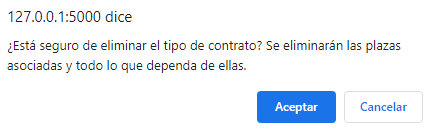
\includegraphics[width=.6\textwidth]{../img/Anexos/Manual usuario/alertElContrato.png}
	\caption{Alerta de eliminación de tipo de contrato}\label{pag:alertElContrato}
\end{figure}


\subsubsection{Creación de áreas}
La creación de nuevas áreas se realiza desde la página principal de áreas.
Para acceder a esta página se debe pulsar sobre la opción del menú llamada <<Áreas>> que se encuentra dentro de la opción desplegable llamada <<Mantenimiento de profesorado>>.

Al acceder a la página principal de áreas (ver imagen~\ref{pag:areas}) se debe pulsar sobre el botón <<Nuevo>>, lo que nos dirigirá al formulario de creación de áreas (imagen~\ref{pag:formArea}).

\begin{figure}
	\centering
	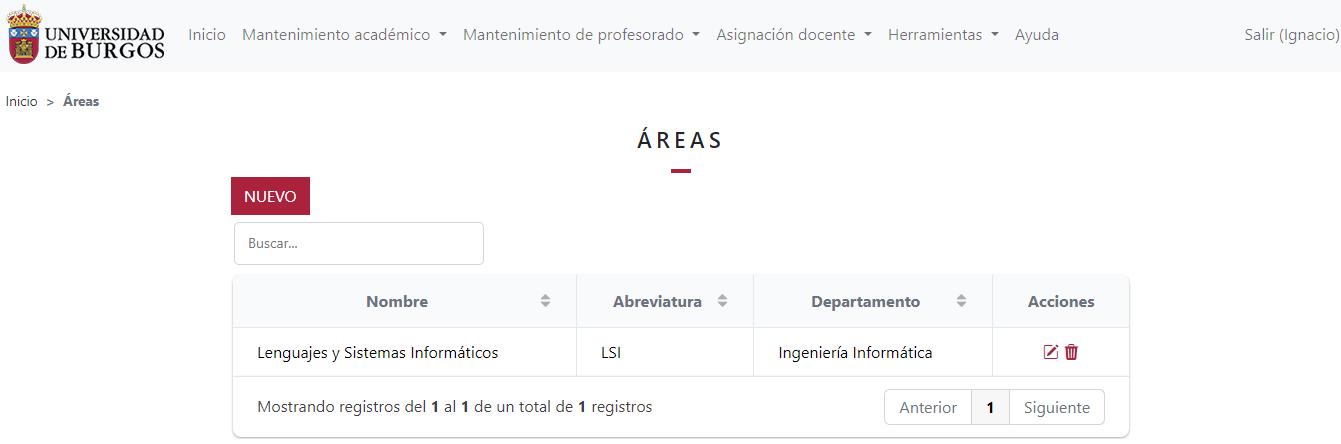
\includegraphics[width=\textwidth]{../img/Anexos/Manual usuario/areas.png}
	\caption{Página principal de áreas}\label{pag:areas}
\end{figure}

\begin{figure}
	\centering
	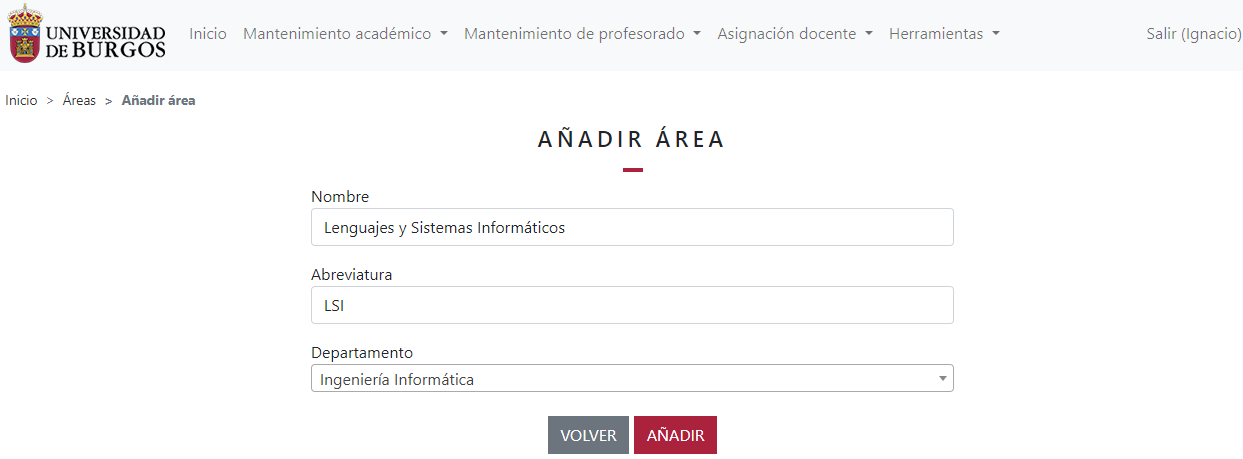
\includegraphics[width=\textwidth]{../img/Anexos/Manual usuario/formArea.png}
	\caption{Formulario de creación de áreas}\label{pag:formArea}
\end{figure}

En este formulario se deben ingresar los datos del área que se desea crear y, una vez este completo, pulsar sobre el botón <<Añadir>>.

Una vez realizado este proceso el área se habrá almacenado en la base de datos y la web nos redirigirá a la página principal de áreas mostrando un mensaje con información sobre la creación.

\subsubsection{Modificación de áreas}
Si necesitamos modificar la información de un área debemos dirigirnos a la página principal de áreas y pulsar sobre el icono del lápiz del área que se desea actualizar.
Pulsar sobre el icono hará que la web nos redireccione a la página que contiene el formulario de modificación del área (imagen~\ref{pag:formModArea}).

\begin{figure}
	\centering
	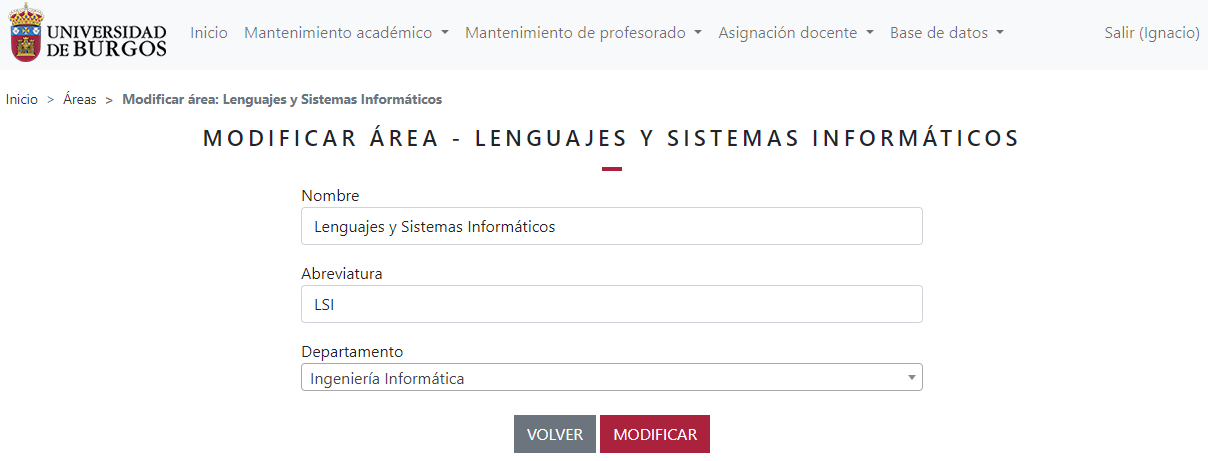
\includegraphics[width=\textwidth]{../img/Anexos/Manual usuario/formModArea.png}
	\caption{Formulario de modificación de áreas}\label{pag:formModArea}
\end{figure}

Desde esta página se pueden editar los campos deseados y, una vez finalice la modificación, pulsar sobre el botón <<Modificar>> para hacer efectivos los cambios.

\subsubsection{Eliminación de áreas}
Para eliminar un área debemos pulsar sobre la opción del menú <<Áreas>> y, una vez en la página principal de áreas, pulsar sobre el icono de la papelera del área que se desea eliminar.

Al realizar esta acción se abrirá una alerta para confirmar la eliminación como la de la imagen~\ref{pag:alertElArea}.

Si se pulsa sobre <<Aceptar>>, se eliminará el área produciendo un borrado en cascada de las plazas dependientes y, por lo tanto, de todo lo relacionado con las plazas.

\begin{figure}
	\centering
	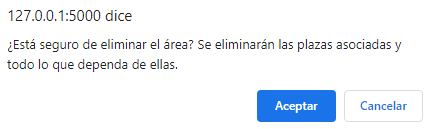
\includegraphics[width=.6\textwidth]{../img/Anexos/Manual usuario/alertElArea.png}
	\caption{Alerta de eliminación de área}\label{pag:alertElArea}
\end{figure}


\subsubsection{Creación de departamentos}
Ante la necesidad de crear un nuevo departamento, debemos desplazarnos al menú de la aplicación web y pulsar sobre la opción llamada <<Departamentos>>. 
Esta acción provocará que se muestre en la pantalla la página principal de los departamentos (ver imagen~\ref{pag:departamentos}), donde se puede ver una tabla con todos los departamentos creados.

Para crear un nuevo departamento se debe pulsar sobre el botón <<Nuevo>>.
Esta acción abrirá una nueva página con el formulario de creación de departamentos (imagen~\ref{pag:formDepartamento}).

Tras rellenar el formulario con los datos del departamento que se desea dar de alta, se debe pulsar sobre el botón <<Añadir>>.
De esta forma el departamento quedará creado y el usuario será redirigido a la página principal de departamentos donde se mostrará un mensaje informativo acerca de la creación realizada.

\begin{figure}
	\centering
	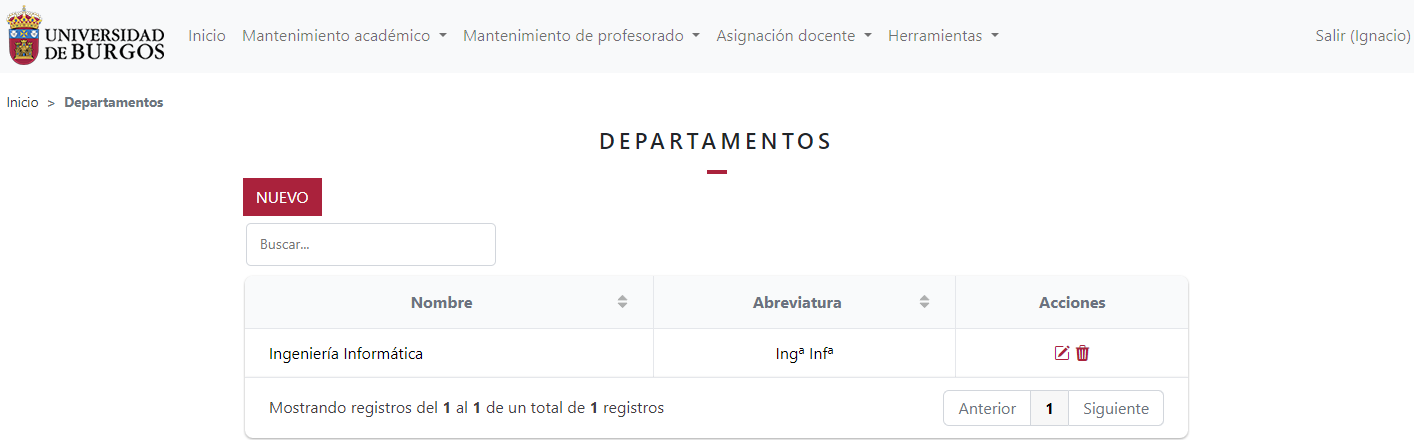
\includegraphics[width=\textwidth]{../img/Anexos/Manual usuario/departamentos.png}
	\caption{Página principal de departamentos}\label{pag:departamentos}
\end{figure}

\begin{figure}
	\centering
	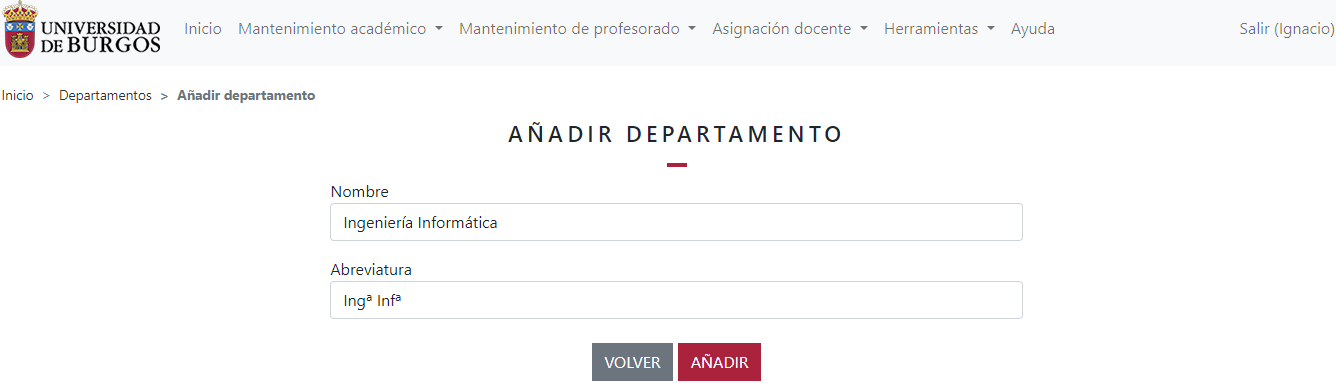
\includegraphics[width=\textwidth]{../img/Anexos/Manual usuario/formDepartamento.png}
	\caption{Formulario de creación de departamentos}\label{pag:formDepartamento}
\end{figure}

\subsubsection{Modificación de departamentos}
Para modificar los datos de un departamento debemos ir a la página principal de departamentos y, una vez ahí, pulsar sobre el icono del lápiz del departamento que se desea actualizar.
Esta acción provocará la redirección al formulario de modificación del departamento que se puede ver en la image~\ref{pag:formModDepartamento}.

Tras modificar los campos deseados, se debe pulsar en el botón <<Modificar>> para hacer los cambios efectivos.
De esta manera, se volverá a la página principal de departamentos donde se verá un mensaje indicando la modificación del departamento.

\begin{figure}
	\centering
	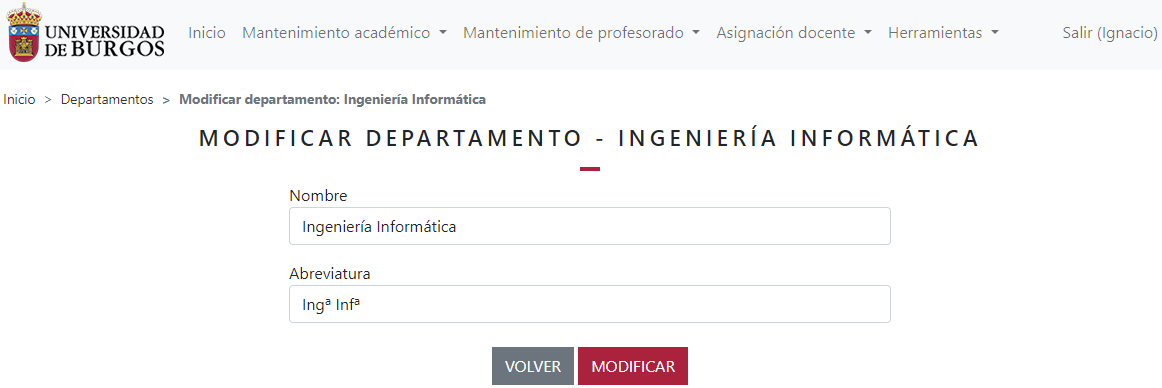
\includegraphics[width=\textwidth]{../img/Anexos/Manual usuario/formModDepartamento.png}
	\caption{Formulario de modificación de departamentos}\label{pag:formModDepartamento}
\end{figure}

\subsubsection{Eliminación de departamentos}
Si se desea dar de baja un departamento se debe ir a la página principal de departamentos y pulsar sobre el icono de la papelera del departamento que se desea eliminar.
Esta acción hará que se abra una alerta (imagen~\ref{pag:alertElDepartamento}) desde la que confirmar la eliminación.

Es importante tener en cuenta que la eliminación de un departamento supone eliminar todas las áreas que se encuentran vinculadas a este, y al borrar las áreas, se eliminará todo lo que se relacione o dependa de ellas.

\begin{figure}
	\centering
	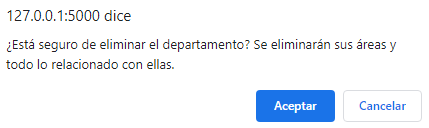
\includegraphics[width=.6\textwidth]{../img/Anexos/Manual usuario/alertElDepartamento.png}
	\caption{Alerta de eliminación de departamento}\label{pag:alertElDepartamento}
\end{figure}

\subsection{Asignación docente}
El apartado de <<Asignación docente>> contiene las herramientas necesarias para la gestión de cursos académicos.
Desde la creación del propio curso, hasta la gestión de grupos y la asignación de plazas a estos grupos.

Para poder acceder a estas funcionalidades, se debe pulsar sobre la opción desplegable del menú llamada <<Asignación docente>> (imagen~\ref{pag:menuAsigDoc}).
Dentro de esta se pueden encontrar las opciones <<Cursos Académicos>>, desde donde realizar la gestión de crear cursos académicos, duplicarlos, añadir asignaturas o eliminarlos, <<Grupos/Horas>>, desde donde se accede a la creación, modificación y eliminación de grupos para las diferentes asignaturas del curso, y <<Horas/Grupos>>, que permite asignar horas que las plazas van a impartir en los diferentes grupos.

\begin{figure}
	\centering
	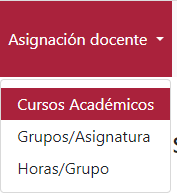
\includegraphics[width=.4\textwidth]{../img/Anexos/Manual usuario/menu asg doc.png}
	\caption{Menú: Asignación docente}\label{pag:menuAsigDoc}
\end{figure}

\subsubsection{Creación de cursos académicos}\label{section:crearCurso}
Para crear un curso académico se debe pulsar sobre la opción del menú llamada <<Cursos Académicos>> que se encuentra dentro del desplegable de asignación docente.
Tras realizar esta acción se abrirá la página de gestión de cursos académicos (ver imagen~\ref{pag:cursos}).

\begin{figure}
	\centering
	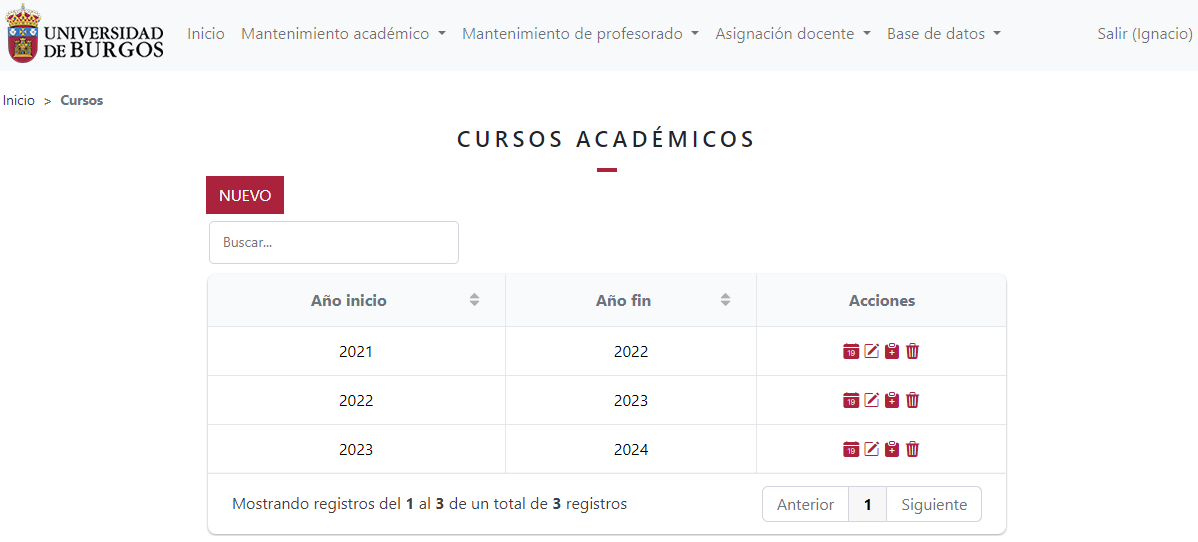
\includegraphics[width=\textwidth]{../img/Anexos/Manual usuario/cursos.png}
	\caption{Página principal de cursos académicos}\label{pag:cursos}
\end{figure}

Una vez en la página, se debe pulsar sobre el botón <<Nuevo>>, lo que nos llevará a la creación de curso, comenzando por una página donde se pide el año de inicio del nuevo curso (imagen~\ref{pag:formCurso1}).

\begin{figure}
	\centering
	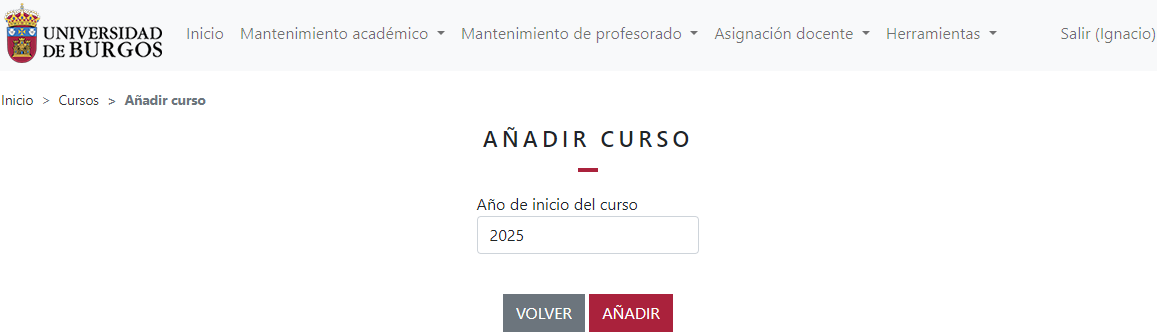
\includegraphics[width=\textwidth]{../img/Anexos/Manual usuario/formCurso1.png}
	\caption{Formulario de creación de curso: año}\label{pag:formCurso1}
\end{figure}

Tras indicar el año de inicio del nuevo curso y pulsar en el botón <<Añadir>> la web mostrará la página desde la que poder seleccionar el número de alumnos y asignaturas de este nuevo curso (ver imagen~\ref{pag:formCurso2}).

\begin{figure}
	\centering
	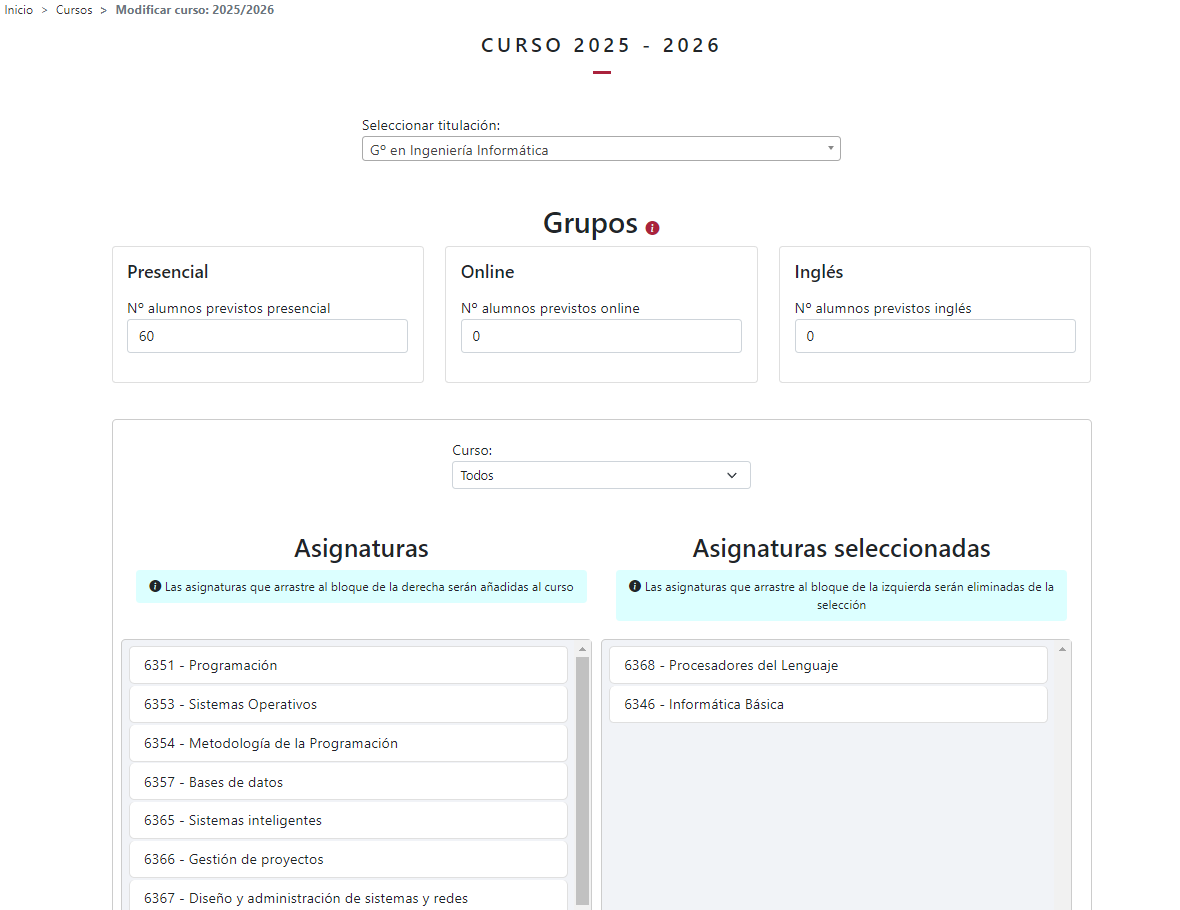
\includegraphics[width=\textwidth]{../img/Anexos/Manual usuario/formCurso2.png}
	\caption{Formulario de creación de curso: selección de asignaturas}\label{pag:formCurso2}
\end{figure}

La forma de trabajar en esta pantalla es la siguiente: 
\begin{enumerate}
\item Seleccionar una titulación en el cuadro de búsqueda llamado <<Seleccionar titulación>>.
\item Indicar el número de alumnos por cada modalidad.

Es necesario indicar el número de alumnos, ya que si se deja vacío, aunque se añadan asignaturas, no se creará la vinculación. No es necesaria poner un número de alumnos a todas la modalidades, sólo a las que se quieran añadir.
\item En la parte de abajo, seleccionar el curso de la titulación desde el campo <<Curso>> si se desea hacer un mayor filtro de búsqueda de asignaturas.
\item En el recuadro con título <<Asignaturas>> aparecerán todas las asignaturas, de la titulación y cursos seleccionados previamente.
Estas asignaturas pueden ser arrastradas con el ratón del bloque izquierdo al bloque derecho, llamado <<Asignaturas seleccionadas>>, para que se añadan al curso académico.

Se pueden ir seleccionando las asignaturas de una en una o pinchar sobre varias, que se pondrán con un fondo verde, y arrastrar la selección completa al bloque derecho.
\end{enumerate}

Una vez se tengan seleccionadas todas las asignaturas que se quieren añadir al curso, y tras haber indicado el número de alumnos por modalidad deseado, se debe pulsar sobre el botón que se encuentra al final de la pantalla llamado <<Añadir>>.

Realizar esta acción producirá la vinculación de las asignaturas seleccionadas con el curso académico creado.
Además, se creará un grupo de teoría y un grupo de práctica para cada asignatura en todas las modalidades donde se haya indicado un número de alumnos mayor a 0.

Al final del proceso, la web mostrará la página principal de cursos con un mensaje como el de la imagen~\ref{pag:mensajeCursoNuevo} si todo ha ido bien.

\begin{figure}
	\centering
	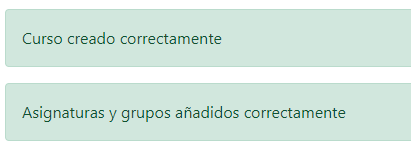
\includegraphics[width=.5\textwidth]{../img/Anexos/Manual usuario/mensajeCursoNuevo.png}
	\caption{Mensaje de creación correcta de curso}\label{pag:mensajeCursoNuevo}
\end{figure}

\subsubsection{Duplicar curso académico}
Para duplicar un curso académico, se debe ir a la página principal de cursos y, desde ahí, pulsar sobre el icono de la imagen~\ref{pag:icnDuplicarCurso} del curso que se desea duplicar.
\begin{figure}
	\centering
	
\includegraphics[width=.08\textwidth]{../img/Anexos/Manual usuario/icnDuplicarCurso.png}
	\caption{Icono de duplicar curso}\label{pag:icnDuplicarCurso}
\end{figure}

Al pulsar sobre el icono se abre una ventana flotante de alerta de confirmación (ver imagen~\ref{pag:alertCurso1}) en la que se pregunta si se está seguro de duplicar el curso.
Al pulsar en <<Aceptar>>, aparecerá la alerta de la imagen~\ref{pag:alertCurso2} en la que se pregunta si se desean duplicar también las plazas asociadas a los diferentes grupos de las asignaturas del curso.

Si se pulsa en <<Aceptar>>, se duplicará el curso exactamente igual que está, con todas las plazas asignadas a los grupos. 
Si se pulsa en <<Cancelar>> sólo de duplicará el curso junto a las asignaturas y grupos.

\begin{figure}
	\centering
	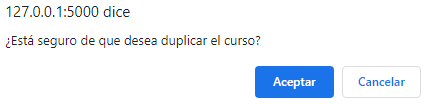
\includegraphics[width=.7\textwidth]{../img/Anexos/Manual usuario/alertCurso1.png}
	\caption{Alerta de duplicar el curso 1}\label{pag:alertCurso1}
\end{figure}

\begin{figure}
	\centering
	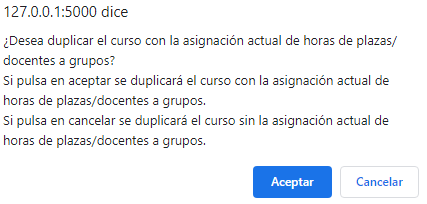
\includegraphics[width=.7\textwidth]{../img/Anexos/Manual usuario/alertCurso2.png}
	\caption{Alerta de duplicar el curso 2}\label{pag:alertCurso2}
\end{figure}

\subsubsection{Añadir asignaturas a un curso académico}
Si después de haber creado un curso se quieren añadir nuevas asignaturas a este, se debe ir a la página principal de cursos y pulsar sobre el icono del lápiz del curso deseado.

Una vez hecho esto, se abrirá la misma página que se utilizaba para la vinculación de asignaturas durante la creación (imagen~\ref{pag:formCurso2}).
El funcionamiento es el mismo (consultar sección \hyperref[section:crearCurso]{<<Creación de cursos académicos>>} para ver como añadir asignaturas a un curso académico).

\subsubsection{Eliminar curso académico}
La eliminación de un curso académico desde la aplicación web no es lo más recomendable ya que mucha información depende de él y podría producir la eliminación de contenido que no se deseaba borrar.

Por los requerimientos dados a la hora de crear la aplicación se ha dificultado la eliminación de cursos para no producir borrados no deseados, por lo que no se realiza un borrado en cascada y se deberá eliminar a mano todo el contenido que dependa del curso previamente.
Por ello, para eliminar un curso académico, lo recomendable es ponerse en contacto con el administrador de sistemas y eliminarlo directamente desde la base de datos de una forma rápida.

Aun así, para eliminar un curso académico desde la aplicación se debe ir a la página principal de cursos y, una vez ahí, pulsar sobre el icono de la papelera del curso deseado.

Esta acción mostrará por pantalla una alerta de confirmación como la de la imagen~\ref{pag:alertElCurso}, donde se informa de que no se podrá eliminar si tiene asignaturas vinculadas.

Si se pulsar sobre <<Aceptar>> y el curso tiene asignaturas vinculadas, se mosrará un mensaje de error como el de la imagen~\ref{pag:menErrorElCurso}. 
En caso contrario, se mostrará un mensaje informando de la eliminación.

\begin{figure}
	\centering
	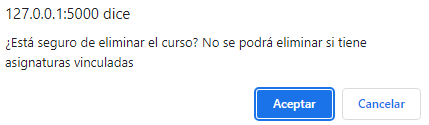
\includegraphics[width=.7\textwidth]{../img/Anexos/Manual usuario/alertElCurso.png}
	\caption{Alerta de eliminación de curso académico}\label{pag:alertElCurso}
\end{figure}

\begin{figure}
	\centering
	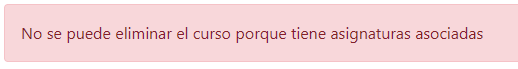
\includegraphics[width=.7\textwidth]{../img/Anexos/Manual usuario/menErrorElCurso.png}
	\caption{Mensaje de error en la eliminación de un curso académico}\label{pag:menErrorElCurso}
\end{figure}

\subsubsection{Crear grupos en una asignatura de un curso académico}
Las asignaturas de un curso académico se encuentran organizadas mediante grupos, donde se distribuye a los alumnos y distintos profesores imparten docencia.

Para poder crear estos grupos a través de la aplicación web es necesario desplazarse a la opción del menú llamada <<Grupos/Asignaturas>> que se encuentra dentro del desplegable llamado <<Asignación docente>>.
Al pulsar sobre esta opción, la web mostrará la página principal de grupos (ver imagen~\ref{pag:grupos}).

\begin{figure}
	\centering
	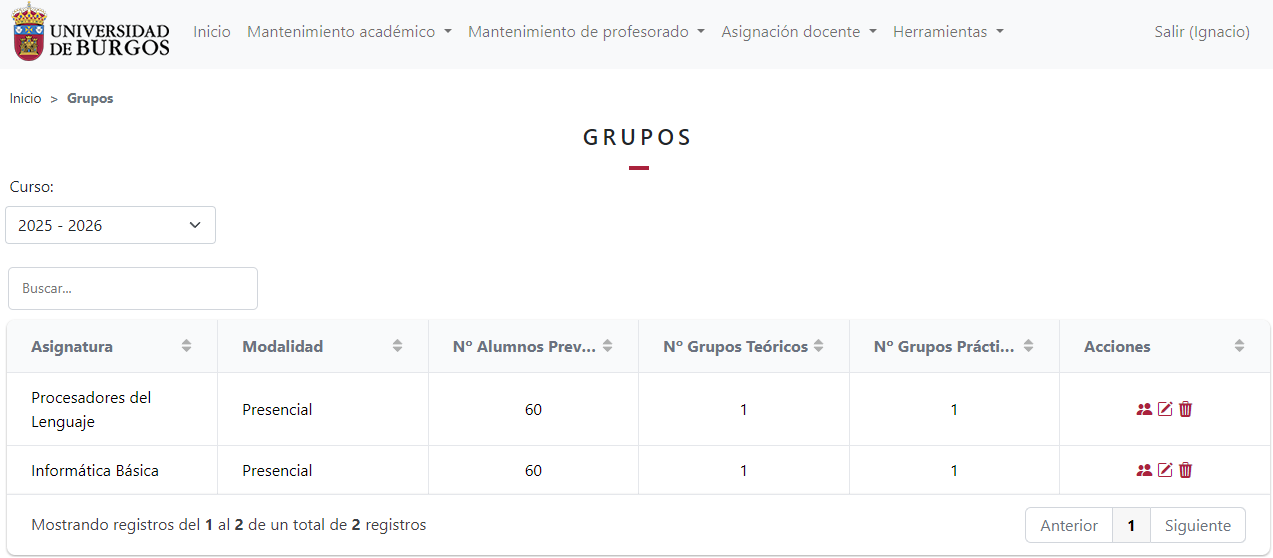
\includegraphics[width=\textwidth]{../img/Anexos/Manual usuario/grupos.png}
	\caption{Página principal de grupos}\label{pag:grupos}
\end{figure}

Desde esta página se debe seleccionar el curso académico sobre el que se quiere trabajar desde el selector de cursos que se encuentra arriba a la izquierda.

Con el curso seleccionado se debe pulsar sobre el icono de las dos personas (imagen~\ref{pag:icnGestionGrupos}) de la asignatura del curso a la que se le quiere añadir un grupo.
Al realizar esta acción, se abrirá la página de gestión de grupos para esa asignatura (ver imagen~\ref{pag:gestionGrupos}).

\begin{figure}
	\centering
	
\includegraphics[width=.07\textwidth]{../img/Anexos/Manual usuario/icnGestionGrupos.png}
	\caption{Icono de gestión de grupos}\label{pag:icnGestionGrupos}
\end{figure}

\begin{figure}
	\centering
	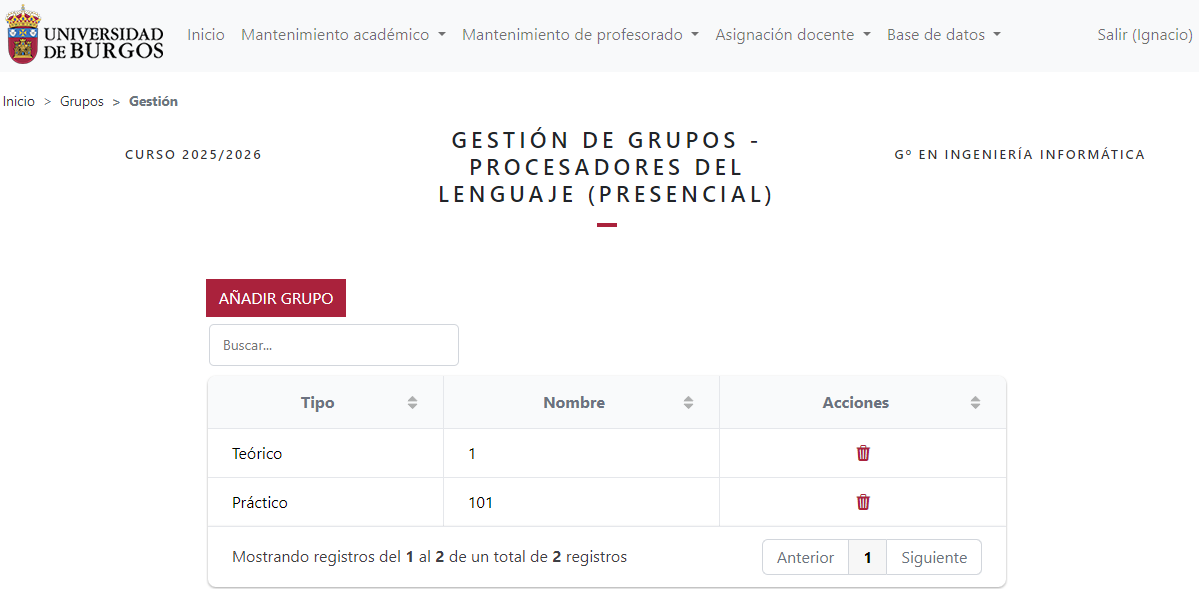
\includegraphics[width=\textwidth]{../img/Anexos/Manual usuario/gestionGrupos.png}
	\caption{Página de gestión de grupos}\label{pag:gestionGrupos}
\end{figure}

Desde la página de gestión se debe pulsar sobre el botón <<Añadir grupo>>, lo que abrirá una ventana flotante desde la que se podrá seleccionar el tipo de grupo a crear (ver imagen~\ref{pag:flotanteNuevoGrupo})

\begin{figure}
	\centering
	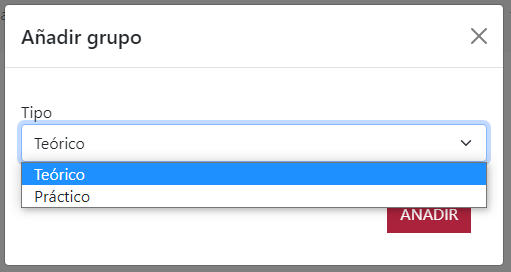
\includegraphics[width=.8\textwidth]{../img/Anexos/Manual usuario/flotanteNuevoGrupo.png}
	\caption{Ventana flotante de creación de grupos}\label{pag:flotanteNuevoGrupo}
\end{figure}

Con el tipo de grupo seleccionado se debe pulsar sobre el botón <<Añadir>>.
De esta manera la ventana flotante se cerrará y el grupo quedará creado con el nombre que le corresponda.

El nombre del grupo se asigna de forma automática siguiendo la relación que deben tener los nombres de grupo, y en el caso de grupos prácticos, su <<división>> por grupos teóricos.

\subsubsection{Eliminar un grupo de una asignatura}\label{section:eliminarGrupo}
Para realizar la eliminación de un grupo de una asignatura se debe acceder a la página de gestión de grupos de esa asignatura (imagen~\ref{pag:gestionGrupos}), y desde ahí, pulsar en el icono de la papelera del grupo que se desea eliminar.

Esta acción producirá la apertura de una alerta de confirmación de la eliminación.
Al pulsar en <<Aceptar>> el grupo quedará eliminado.

Existen algunas excepciones que no permiten eliminar un grupo:
\begin{itemize}
\item Se trata del único grupo de teoría y existen grupos prácticos:
En caso de querer eliminar el único grupo de teoría existente, pero tener algún grupo práctico que dependa de él, no se podrá eliminar, habrá que eliminar antes los grupos prácticos.
\item Grupo con vinculaciones a alguna plaza:
Si el grupo que se intenta eliminar tiene alguna vinculación con una o más plazas, no se podrá eliminar directamente, habrá que eliminar primero las vinculaciones.
\end{itemize}

Esa información se mostrará si el grupo se encuentra bajo alguna de estas excepciones, si no, aparecerá un mensaje indicando la correcta eliminación y el grupo desaparecerá de la lista.

\subsubsection{Eliminación de una asignatura del curso}\label{section:eliminarAsigCurso}
Para eliminar una asignatura de un curso académico hay que dirigirse a la página principal de grupos/asignaturas (ver imagen~\ref{pag:grupos}), a la que se accede desde la opción del mení <<Grupos/Asignatura>>.

Desde esta página se debe elegir el curso académico sobre el que se quiere trabajar desde el seleccionador de cursos de la parte superior izquierda.
Tras hacer esto, aparecerá un listado con todas las asignaturas del curso académico.

Para eliminar una asignatura se debe pulsar sobre el icono de la papelera de la asignatura deseada.
Esto abrirá una alerta para confirmar la eliminación (imagen~\ref{pag:alertElAsigCurso}).

\begin{figure}
	\centering
	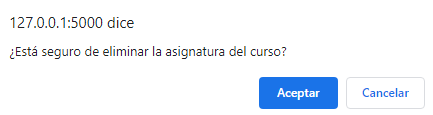
\includegraphics[width=.7\textwidth]{../img/Anexos/Manual usuario/alertElAsigCurso.png}
	\caption{Alerta de eliminación de asignatura del curso académico}\label{pag:alertElAsigCurso}
\end{figure}

Al pulsar en <<Aceptar>>, si todo va bien, se eliminará la asignatura del curso y aparecerá un mensaje indicando la acción realizada.
En caso contrario, se mostrará un mensaje con el error producido.

Las excepciones que no permiten eliminar una asignatura del curso directamente son las siguientes:
\begin{itemize}
\item La asignatura tiene grupos vinculados:
En este caso se deben eliminar los grupos previamente. 
Se puede ver como eliminar un grupo en la sección \hyperref[section:eliminarGrupo]{<<Eliminar un grupo de una asignatura>>}.
\item La asignatura tiene algún grupo previsto:
Esta información se puede ver y modificar pulsando sobre el icono del lápiz de la asignatura.
Ahí se debe indicar el número 0 tanto para grupos prácticos como teóricos previstos.
De esta forma, se evitará esta excepción.
\end{itemize}

\subsubsection{Modificar información de una asignatura de un curso académico}
Desde la página principal de grupos/asignaturas de un curso (imagen~\ref{pag:grupos}) se puede modificar la información de alumnos y grupos previstos.

Para realizar esta acción se debe pulsar sobre el icono del lápiz de la asignatura del curso a editar. 
Esto abrirá una ventana flotante como la de la imagen~\ref{pag:flotanteEditarAsig} desde donde se pueden indicar, tanto el número de alumnos previstos, como el de grupos teóricos y prácticos previstos.

Tras realizar los cambios, pulsar en el botón <<Modificar>> producirá la actualización de estos datos.

Es importante saber que estos datos sólo tienen carácter informativo, y que ningún elemento de la aplicación depende de ellos. Aun así, el número previsto de grupos prácticos y teóricos sí que influye en la eliminación de las asignaturas de curso, ya que se considera, que si tiene grupos previstos no debería eliminarse del curso.

La información completa sobre la eliminación de asignaturas de un curso académico se puede ver en la sección \hyperref[section:eliminarAsigCurso]{<<Eliminación de una asignatura del curso>>}.

\begin{figure}
	\centering
	\includegraphics[width=.65\textwidth]{../img/Anexos/Manual usuario/flotanteEditarAsig.png}
	\caption{Ventana flotante de editar asignatura del curso académico}\label{pag:flotanteEditarAsig}
\end{figure}

\subsubsection{Asignar horas de una plaza a un grupo}
La asignación de horas de plazas a grupos se realiza desde la página principal de horas de un curso académico (ver imagen~\ref{pag:horas}).

\begin{figure}
	\centering
	\includegraphics[width=\textwidth]{../img/Anexos/Manual usuario/horas.png}
	\caption{Página principal de horas de grupos}\label{pag:horas}
\end{figure}

Para acceder a esta página se debe pulsar sobre la opción del menú llamada <<Horas/Grupo>>, que se encuentra dentro de la opción desplegable del menú llamada <<Asignación docente>>.

Una vez en la página principal de horas, se debe seleccionar un curso académico desde el selector de cursos que se encuentra en la parte superior izquierda.

Al seleccionar el curso, se mostrará el listado completo de grupos que tiene el curso académico.

Para asignar una plaza a un grupo se debe pulsar sobre el icono del reloj (imagen~\ref{pag:icnHoras}) del grupo de la tabla al que se le desea añadir horas de una plaza.

\begin{figure}
	\centering
	\includegraphics[width=.07\textwidth]{../img/Anexos/Manual usuario/icnHoras.png}
	\caption{Página principal de horas de grupos}\label{pag:icnHoras}
\end{figure}

Tras pulsar en el icono, se abrirá la página de gestión de horas del grupo (ver imagen~\ref{pag:horasGrupo}).

\begin{figure}
	\centering
	\includegraphics[width=\textwidth]{../img/Anexos/Manual usuario/horasGrupo.png}
	\caption{Página de gestión de horas de un grupo}\label{pag:horasGrupo}
\end{figure}

Pulsando en el botón <<Añadir Plaza>> se abre una ventana flotante (ver imagen~\ref{pag:flotanteAddPlaza}) en la que se puede seleccionar la plaza que se quiere vincular y el número de horas de docencia que va a impartir.

\begin{figure}
	\centering
	\includegraphics[width=.7\textwidth]{../img/Anexos/Manual usuario/flotanteAddPlaza.png}
	\caption{Ventana flotante de vincular una plaza a un grupo}\label{pag:flotanteAddPlaza}
\end{figure}

Con la plaza seleccionada y las horas indicadas, se debe pulsar sobre el botón <<Añadir>> para que se cree la vinculación de la plaza con el grupo.

Al realizar esta acción la ventana flotante se cerrará y se informará mediante un mensaje sobre la vinculación entre la plaza y el grupo.

\subsubsection{Asignar horas desde la tabla de horas}
Para agilizar el trabajo de modificar las horas que una plaza tiene asignadas a un grupo, se puede acceder a la página principal de horas de un curso académico (ver imagen~\ref{pag:horas}), donde aparecerá la tabla con los grupos del curso académico junto a las plazas asignadas a dichos grupos.

En esta tabla aparecerán, como máximo, tres de las plazas asignadas al grupo junto a las horas que va a impartir en dicho grupo y la información de horas totales asignadas, en ese y otros grupos.

Las columnas de la tabla llamadas <<Horas en el grupo>> se pueden modificar si tienen una plaza asignada.
Para ello, se debe pulsar sobre la celda y se podrá escribir el número de horas.
Al salir de la celda, el dato se actualizará automáticamente y aparecerá un mensaje informando de la modificación realizada.

Para navegar por la tabla se puede hacer mediante el ratón pulsando en las diferentes celdas o mediante la tecla <<Tabulador>> del teclado. Además, se puede <<salir>> de la celda pulsando fuera de ella o pulsando la tecla <<ENTER>> del teclado.
Esta forma de salir de la celda hará efectivo el cambio realizado.

Por último, también se puede <<salir>> sin hacer efectivos los cambios de la celda pulsando la tecla <<ESC>> del teclado.

\subsection{Base de datos}
La aplicación web cuenta con un sistema que permite exportar los datos de la base de datos y, también, hacer importaciones de datos.

El acceso a estas herramientas se realiza desde el menú de la web, pulsando sobre la opción desplegable llamada <<Base de datos>>, que se puede ver en la imagen~\ref{pag:menu bd}.

\begin{figure}
	\centering
	\includegraphics[width=.35\textwidth]{../img/Anexos/Manual usuario/menu bd.png}
	\caption{Menú: Base de datos}\label{pag:menu bd}
\end{figure}

\subsubsection{Exportar la información de la base de datos}
Para exportar los datos que se encuentran en la base de datos se debe pulsar sobre la opción del menú llamada <<Exportar>> que se encuentra dentro del desplegable llamado <<Base de datos>>.

Al pulsar sobre la opción se descargará automáticamente en el dispositivo del usuario un archivo \texttt{SQL} con los datos que contiene la base de datos en sentencias \texttt{INSERT} que permitirán importar de nuevo los datos en la web.

\subsubsection{Importar datos a la base de datos}
El acceso a esta herramienta se realiza pulsando sobre la opción del menú llamada <<Importar>>, que se encuentra dentro de la opción llamada <<Base de datos>>.

Al realizar esta acción se accede a la página de importación de los datos (ver imagen~\ref{pag:importar}).

Desde esta página se debe seleccionar el archivo que contiene los datos a importar.
Este archivo debe ser de tipo \texttt{SQL} y sólo debe contener sentencias de tipo \texttt{INSERT}, cualquier otro tipo de sentencia no será aceptada y, por lo tanto, no se permitirá el uso del archivo.

Es importante saber que el uso de esta herramienta puede afectar al contenido de la base de datos, por lo que es recomendable hacer una copia de seguridad previamente si se tienen datos importantes que se pueden querer recuperar en caso de que algo falle.

Al importar los datos se elimina todo el contenido que esté en ese momento en la base de datos y se almacenan los datos del archivo subido.

Cuando se realiza la importación, se cierra la sesión que estuviese abierta y se redirige a la página de inicio de sesión, donde aparecerá un mensaje indicando el resultado de la importación.

\begin{figure}
	\centering
	\includegraphics[width=\textwidth]{../img/Anexos/Manual usuario/importar.png}
	\caption{Página de importación de datos}\label{pag:importar}
\end{figure}

